\documentclass[a4paper]{book}
\usepackage{makeidx}
\usepackage{natbib}
\usepackage{graphicx}
\usepackage{multicol}
\usepackage{float}
\usepackage{listings}
\usepackage{color}
\usepackage{ifthen}
\usepackage[table]{xcolor}
\usepackage{textcomp}
\usepackage{alltt}
\usepackage{ifpdf}
\ifpdf
\usepackage[pdftex,
            pagebackref=true,
            colorlinks=true,
            linkcolor=blue,
            unicode
           ]{hyperref}
\else
\usepackage[ps2pdf,
            pagebackref=true,
            colorlinks=true,
            linkcolor=blue,
            unicode
           ]{hyperref}
\usepackage{pspicture}
\fi
\usepackage[utf8]{inputenc}
\usepackage{mathptmx}
\usepackage[scaled=.90]{helvet}
\usepackage{courier}
\usepackage{sectsty}
\usepackage[titles]{tocloft}
\usepackage{doxygen}
\lstset{language=C++,inputencoding=utf8,basicstyle=\footnotesize,breaklines=true,breakatwhitespace=true,tabsize=8,numbers=left }
\makeindex
\setcounter{tocdepth}{3}
\renewcommand{\footrulewidth}{0.4pt}
\renewcommand{\familydefault}{\sfdefault}
\hfuzz=15pt
\setlength{\emergencystretch}{15pt}
\hbadness=750
\tolerance=750
\begin{document}
\hypersetup{pageanchor=false,citecolor=blue}
\begin{titlepage}
\vspace*{7cm}
\begin{center}
{\Large \-O\-R\-M\-C++ \\[1ex]\large 0.\-1 }\\
\vspace*{1cm}
{\large \-Generated by Doxygen 1.7.5.1}\\
\vspace*{0.5cm}
{\small Fri May 11 2012 01:43:26}\\
\end{center}
\end{titlepage}
\clearemptydoublepage
\pagenumbering{roman}
\tableofcontents
\clearemptydoublepage
\pagenumbering{arabic}
\hypersetup{pageanchor=true,citecolor=blue}
\chapter{\-Class \-Index}
\section{\-Class \-Hierarchy}
\-This inheritance list is sorted roughly, but not completely, alphabetically\-:\begin{DoxyCompactList}
\item \contentsline{section}{ormcore\-:\-:\-O\-C\-Object}{\pageref{classormcore_1_1_o_c_object}}{}
\begin{DoxyCompactList}
\item \contentsline{section}{ormcore\-:\-:\-O\-C\-Application}{\pageref{classormcore_1_1_o_c_application}}{}
\item \contentsline{section}{ormcore\-:\-:\-O\-C\-D\-B\-Manager}{\pageref{classormcore_1_1_o_c_d_b_manager}}{}
\item \contentsline{section}{ormcore\-:\-:\-O\-C\-D\-B\-Object$<$ \-T $>$}{\pageref{classormcore_1_1_o_c_d_b_object}}{}
\item \contentsline{section}{ormcore\-:\-:\-O\-C\-Exception}{\pageref{classormcore_1_1_o_c_exception}}{}
\begin{DoxyCompactList}
\item \contentsline{section}{ormcore\-:\-:\-O\-C\-File\-Exception}{\pageref{classormcore_1_1_o_c_file_exception}}{}
\item \contentsline{section}{ormcore\-:\-:\-O\-C\-S\-Q\-L\-Exception}{\pageref{classormcore_1_1_o_c_s_q_l_exception}}{}
\end{DoxyCompactList}
\item \contentsline{section}{ormcore\-:\-:\-O\-C\-Exceptions\-Helper}{\pageref{classormcore_1_1_o_c_exceptions_helper}}{}
\item \contentsline{section}{ormcore\-:\-:\-O\-C\-Logger}{\pageref{classormcore_1_1_o_c_logger}}{}
\item \contentsline{section}{ormcore\-:\-:\-O\-C\-Model}{\pageref{classormcore_1_1_o_c_model}}{}
\begin{DoxyCompactList}
\item \contentsline{section}{ormcore\-:\-:\-O\-C\-Application\-Manager}{\pageref{classormcore_1_1_o_c_application_manager}}{}
\item \contentsline{section}{ormcore\-:\-:\-O\-C\-Parameter}{\pageref{classormcore_1_1_o_c_parameter}}{}
\end{DoxyCompactList}
\end{DoxyCompactList}
\item \contentsline{section}{\-O\-R\-M\-C\-U\-T\-Test}{\pageref{class_o_r_m_c_u_t_test}}{}
\end{DoxyCompactList}

\chapter{\-Class \-Index}
\section{\-Class \-List}
\-Here are the classes, structs, unions and interfaces with brief descriptions\-:\begin{DoxyCompactList}
\item\contentsline{section}{\hyperlink{classormcore_1_1_o_c_application}{ormcore\-::\-O\-C\-Application} }{\pageref{classormcore_1_1_o_c_application}}{}
\item\contentsline{section}{\hyperlink{classormcore_1_1_o_c_application_manager}{ormcore\-::\-O\-C\-Application\-Manager} }{\pageref{classormcore_1_1_o_c_application_manager}}{}
\item\contentsline{section}{\hyperlink{classormcore_1_1_o_c_d_b_manager}{ormcore\-::\-O\-C\-D\-B\-Manager} }{\pageref{classormcore_1_1_o_c_d_b_manager}}{}
\item\contentsline{section}{\hyperlink{classormcore_1_1_o_c_d_b_object}{ormcore\-::\-O\-C\-D\-B\-Object$<$ T $>$} }{\pageref{classormcore_1_1_o_c_d_b_object}}{}
\item\contentsline{section}{\hyperlink{classormcore_1_1_o_c_exception}{ormcore\-::\-O\-C\-Exception} }{\pageref{classormcore_1_1_o_c_exception}}{}
\item\contentsline{section}{\hyperlink{classormcore_1_1_o_c_exceptions_helper}{ormcore\-::\-O\-C\-Exceptions\-Helper} }{\pageref{classormcore_1_1_o_c_exceptions_helper}}{}
\item\contentsline{section}{\hyperlink{classormcore_1_1_o_c_file_exception}{ormcore\-::\-O\-C\-File\-Exception} }{\pageref{classormcore_1_1_o_c_file_exception}}{}
\item\contentsline{section}{\hyperlink{classormcore_1_1_o_c_logger}{ormcore\-::\-O\-C\-Logger} }{\pageref{classormcore_1_1_o_c_logger}}{}
\item\contentsline{section}{\hyperlink{classormcore_1_1_o_c_model}{ormcore\-::\-O\-C\-Model} }{\pageref{classormcore_1_1_o_c_model}}{}
\item\contentsline{section}{\hyperlink{classormcore_1_1_o_c_object}{ormcore\-::\-O\-C\-Object} }{\pageref{classormcore_1_1_o_c_object}}{}
\item\contentsline{section}{\hyperlink{classormcore_1_1_o_c_parameter}{ormcore\-::\-O\-C\-Parameter} }{\pageref{classormcore_1_1_o_c_parameter}}{}
\item\contentsline{section}{\hyperlink{classormcore_1_1_o_c_s_q_l_exception}{ormcore\-::\-O\-C\-S\-Q\-L\-Exception} }{\pageref{classormcore_1_1_o_c_s_q_l_exception}}{}
\item\contentsline{section}{\hyperlink{class_o_r_m_c_u_t_test}{\-O\-R\-M\-C\-U\-T\-Test} }{\pageref{class_o_r_m_c_u_t_test}}{}
\end{DoxyCompactList}

\chapter{\-Class \-Documentation}
\hypertarget{classormcore_1_1_o_c_application}{
\section{ormcore\-:\-:\-O\-C\-Application \-Class \-Reference}
\label{classormcore_1_1_o_c_application}\index{ormcore\-::\-O\-C\-Application@{ormcore\-::\-O\-C\-Application}}
}
\-Inheritance diagram for ormcore\-:\-:\-O\-C\-Application\-:\begin{figure}[H]
\begin{center}
\leavevmode
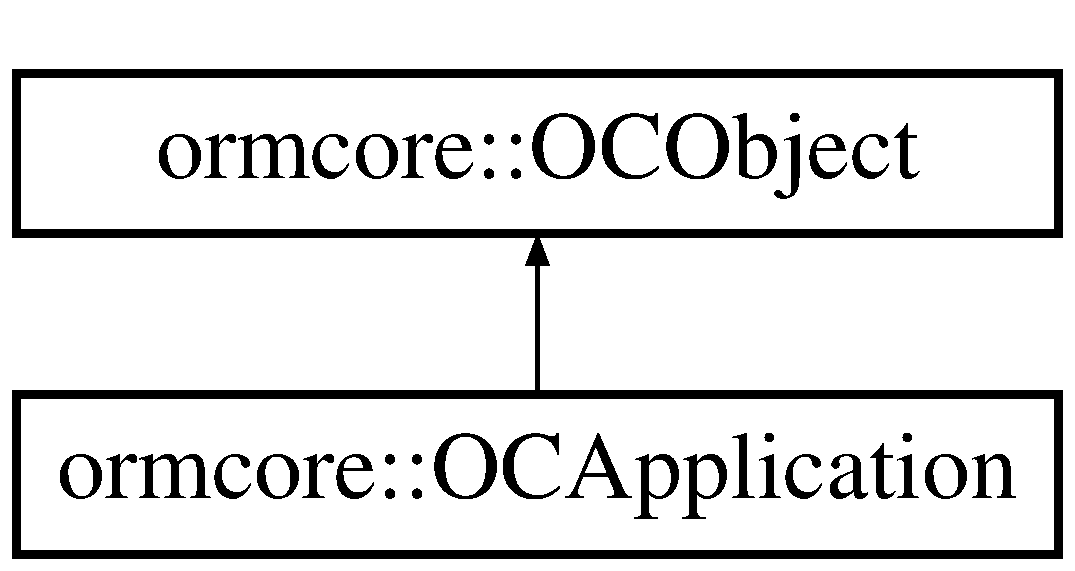
\includegraphics[height=2.000000cm]{classormcore_1_1_o_c_application}
\end{center}
\end{figure}
\subsection*{\-Static \-Public \-Member \-Functions}
\begin{DoxyCompactItemize}
\item 
static bool \hyperlink{classormcore_1_1_o_c_application_a6fe0a11cab9afaa519316e038543341a}{init\-O\-C\-Apllication} (\-Q\-String application\-Name, \-Q\-String application\-Version)
\item 
static bool \hyperlink{classormcore_1_1_o_c_application_a23d0ff096f802d612d589ab93f340d78}{init\-Application\-Manager} (\-Q\-String application\-Name, \-Q\-String application\-Version)
\item 
static void \hyperlink{classormcore_1_1_o_c_application_aa6aa8b5f90f1744c23f968a3f71feab6}{close\-Application\-Manager} ()
\item 
\hypertarget{classormcore_1_1_o_c_application_aa1685b6ed517ac2c13a6232bb0ec7e6f}{
static \hyperlink{classormcore_1_1_o_c_d_b_object}{\-O\-C\-D\-B\-Object}\*
$<$ \hyperlink{classormcore_1_1_o_c_application_manager}{\-O\-C\-Application\-Manager} $>$ {\bfseries application\-Manager} ()}
\label{classormcore_1_1_o_c_application_aa1685b6ed517ac2c13a6232bb0ec7e6f}

\end{DoxyCompactItemize}
\subsection*{\-Static \-Public \-Attributes}
\begin{DoxyCompactItemize}
\item 
\hypertarget{classormcore_1_1_o_c_application_a3c3ae7e118f126824c8c04ca2549764f}{
static \hyperlink{classormcore_1_1_o_c_d_b_object}{\-O\-C\-D\-B\-Object}\*
$<$ \hyperlink{classormcore_1_1_o_c_application_manager}{\-O\-C\-Application\-Manager} $>$ {\bfseries \-\_\-app\-Manager}}
\label{classormcore_1_1_o_c_application_a3c3ae7e118f126824c8c04ca2549764f}

\end{DoxyCompactItemize}


\subsection{\-Member \-Function \-Documentation}
\hypertarget{classormcore_1_1_o_c_application_aa6aa8b5f90f1744c23f968a3f71feab6}{
\index{ormcore\-::\-O\-C\-Application@{ormcore\-::\-O\-C\-Application}!close\-Application\-Manager@{close\-Application\-Manager}}
\index{close\-Application\-Manager@{close\-Application\-Manager}!ormcore::OCApplication@{ormcore\-::\-O\-C\-Application}}
\subsubsection[{close\-Application\-Manager}]{\setlength{\rightskip}{0pt plus 5cm}static void ormcore\-::\-O\-C\-Application\-::close\-Application\-Manager (
\begin{DoxyParamCaption}
{}
\end{DoxyParamCaption}
)\hspace{0.3cm}{\ttfamily  \mbox{[}static\mbox{]}}}}
\label{classormcore_1_1_o_c_application_aa6aa8b5f90f1744c23f968a3f71feab6}
\-Fecha gerenciador da aplicação no banco de dados \hypertarget{classormcore_1_1_o_c_application_a23d0ff096f802d612d589ab93f340d78}{
\index{ormcore\-::\-O\-C\-Application@{ormcore\-::\-O\-C\-Application}!init\-Application\-Manager@{init\-Application\-Manager}}
\index{init\-Application\-Manager@{init\-Application\-Manager}!ormcore::OCApplication@{ormcore\-::\-O\-C\-Application}}
\subsubsection[{init\-Application\-Manager}]{\setlength{\rightskip}{0pt plus 5cm}static bool ormcore\-::\-O\-C\-Application\-::init\-Application\-Manager (
\begin{DoxyParamCaption}
\item[{\-Q\-String}]{application\-Name, }
\item[{\-Q\-String}]{application\-Version}
\end{DoxyParamCaption}
)\hspace{0.3cm}{\ttfamily  \mbox{[}static\mbox{]}}}}
\label{classormcore_1_1_o_c_application_a23d0ff096f802d612d589ab93f340d78}
\-Inicializa gerenciador da aplicação no banco de dados 
\begin{DoxyParams}{\-Parameters}
{\em application\-Name} & \-Q\-String com o nome da aplicação \\
\hline
{\em application\-Version} & \-Q\-String com a versão da aplicação \\
\hline
\end{DoxyParams}
\hypertarget{classormcore_1_1_o_c_application_a6fe0a11cab9afaa519316e038543341a}{
\index{ormcore\-::\-O\-C\-Application@{ormcore\-::\-O\-C\-Application}!init\-O\-C\-Apllication@{init\-O\-C\-Apllication}}
\index{init\-O\-C\-Apllication@{init\-O\-C\-Apllication}!ormcore::OCApplication@{ormcore\-::\-O\-C\-Application}}
\subsubsection[{init\-O\-C\-Apllication}]{\setlength{\rightskip}{0pt plus 5cm}static bool ormcore\-::\-O\-C\-Application\-::init\-O\-C\-Apllication (
\begin{DoxyParamCaption}
\item[{\-Q\-String}]{application\-Name, }
\item[{\-Q\-String}]{application\-Version}
\end{DoxyParamCaption}
)\hspace{0.3cm}{\ttfamily  \mbox{[}static\mbox{]}}}}
\label{classormcore_1_1_o_c_application_a6fe0a11cab9afaa519316e038543341a}
\-Inicializa aplicação, sincronizando dados com o banco 

\-The documentation for this class was generated from the following file\-:\begin{DoxyCompactItemize}
\item 
\-O\-R\-M\-C++/include/ocapplication.\-h\end{DoxyCompactItemize}

\hypertarget{classormcore_1_1_o_c_application_manager}{
\section{ormcore\-:\-:\-O\-C\-Application\-Manager \-Class \-Reference}
\label{classormcore_1_1_o_c_application_manager}\index{ormcore\-::\-O\-C\-Application\-Manager@{ormcore\-::\-O\-C\-Application\-Manager}}
}
\-Inheritance diagram for ormcore\-:\-:\-O\-C\-Application\-Manager\-:\begin{figure}[H]
\begin{center}
\leavevmode
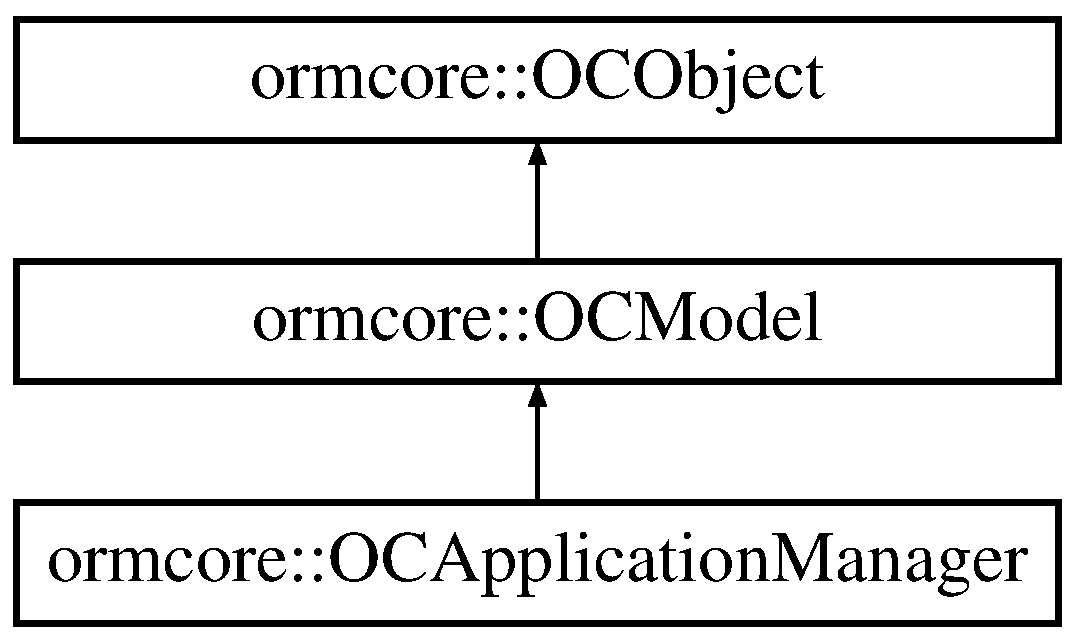
\includegraphics[height=3.000000cm]{classormcore_1_1_o_c_application_manager}
\end{center}
\end{figure}
\subsection*{\-Public \-Member \-Functions}
\begin{DoxyCompactItemize}
\item 
\hyperlink{classormcore_1_1_o_c_application_manager_ae9f11ee127603b9e35fd40d99620a293}{\-O\-C\-Application\-Manager} ()
\end{DoxyCompactItemize}
\subsection*{\-Static \-Public \-Attributes}
\begin{DoxyCompactItemize}
\item 
\hypertarget{classormcore_1_1_o_c_application_manager_adc5e1351b917d025c0d34ec513f99bbf}{
static \-Q\-String {\bfseries \-\_\-full\-Schema}}
\label{classormcore_1_1_o_c_application_manager_adc5e1351b917d025c0d34ec513f99bbf}

\item 
\hypertarget{classormcore_1_1_o_c_application_manager_aed2df83911c3b30b50b27e0c85898314}{
static \-Q\-String {\bfseries \-\_\-table\-Name}}
\label{classormcore_1_1_o_c_application_manager_aed2df83911c3b30b50b27e0c85898314}

\end{DoxyCompactItemize}


\subsection{\-Constructor \& \-Destructor \-Documentation}
\hypertarget{classormcore_1_1_o_c_application_manager_ae9f11ee127603b9e35fd40d99620a293}{
\index{ormcore\-::\-O\-C\-Application\-Manager@{ormcore\-::\-O\-C\-Application\-Manager}!\-O\-C\-Application\-Manager@{\-O\-C\-Application\-Manager}}
\index{\-O\-C\-Application\-Manager@{\-O\-C\-Application\-Manager}!ormcore::OCApplicationManager@{ormcore\-::\-O\-C\-Application\-Manager}}
\subsubsection[{\-O\-C\-Application\-Manager}]{\setlength{\rightskip}{0pt plus 5cm}ormcore\-::\-O\-C\-Application\-Manager\-::\-O\-C\-Application\-Manager (
\begin{DoxyParamCaption}
{}
\end{DoxyParamCaption}
)}}
\label{classormcore_1_1_o_c_application_manager_ae9f11ee127603b9e35fd40d99620a293}
\-Construtor de \hyperlink{classormcore_1_1_o_c_application_manager}{\-O\-C\-Application\-Manager} 

\-The documentation for this class was generated from the following file\-:\begin{DoxyCompactItemize}
\item 
\-O\-R\-M\-C++/include/ocapplicationmanager.\-h\end{DoxyCompactItemize}

\hypertarget{classormcore_1_1_o_c_d_b_manager}{
\section{ormcore\-:\-:\-O\-C\-D\-B\-Manager \-Class \-Reference}
\label{classormcore_1_1_o_c_d_b_manager}\index{ormcore\-::\-O\-C\-D\-B\-Manager@{ormcore\-::\-O\-C\-D\-B\-Manager}}
}
\-Inheritance diagram for ormcore\-:\-:\-O\-C\-D\-B\-Manager\-:\begin{figure}[H]
\begin{center}
\leavevmode
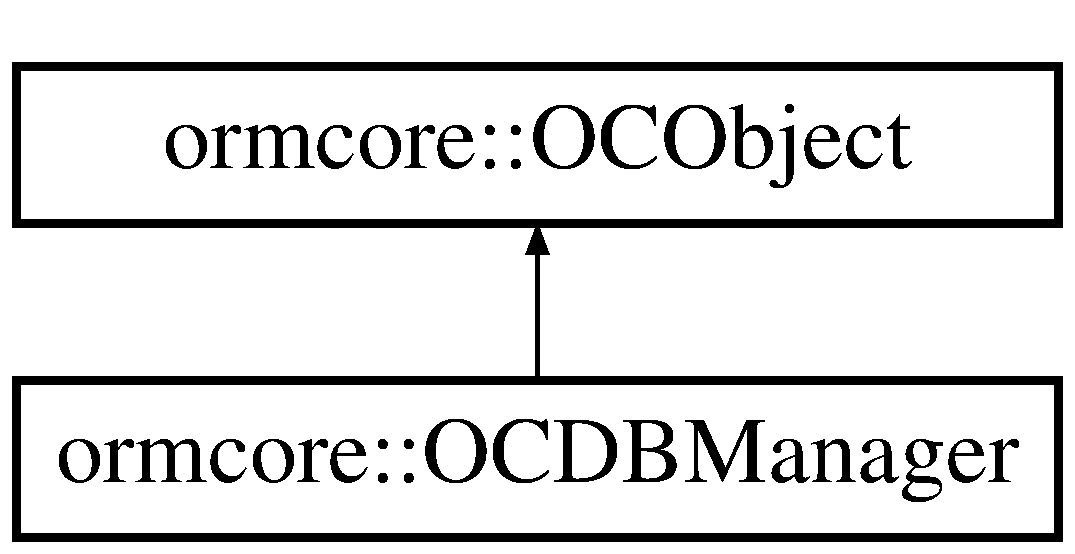
\includegraphics[height=2.000000cm]{classormcore_1_1_o_c_d_b_manager}
\end{center}
\end{figure}
\subsection*{\-Static \-Public \-Member \-Functions}
\begin{DoxyCompactItemize}
\item 
static void \hyperlink{classormcore_1_1_o_c_d_b_manager_a30fc8cd88de7ff50e1d0c3fd3be99451}{set\-Data\-Base\-Name} (const \-Q\-String database\-Name)
\item 
static void \hyperlink{classormcore_1_1_o_c_d_b_manager_a5c5f905f5b91f9018d4fbd047e5aaa93}{connect} ()
\item 
static void \hyperlink{classormcore_1_1_o_c_d_b_manager_ac1425506ca2714cf62528bf48e4e372b}{close} ()
\item 
static void \hyperlink{classormcore_1_1_o_c_d_b_manager_a6482ce90b6c3f937f3e5aec74173cade}{drop} ()
\end{DoxyCompactItemize}
\subsection*{\-Static \-Public \-Attributes}
\begin{DoxyCompactItemize}
\item 
\hypertarget{classormcore_1_1_o_c_d_b_manager_ae8f27a1a41d27e0cfc4ba5bea99811e5}{
static \-Q\-Sql\-Database {\bfseries \-\_\-db} = \-Q\-Sql\-Database()}
\label{classormcore_1_1_o_c_d_b_manager_ae8f27a1a41d27e0cfc4ba5bea99811e5}

\end{DoxyCompactItemize}


\subsection{\-Member \-Function \-Documentation}
\hypertarget{classormcore_1_1_o_c_d_b_manager_ac1425506ca2714cf62528bf48e4e372b}{
\index{ormcore\-::\-O\-C\-D\-B\-Manager@{ormcore\-::\-O\-C\-D\-B\-Manager}!close@{close}}
\index{close@{close}!ormcore::OCDBManager@{ormcore\-::\-O\-C\-D\-B\-Manager}}
\subsubsection[{close}]{\setlength{\rightskip}{0pt plus 5cm}void \-O\-C\-D\-B\-Manager\-::close (
\begin{DoxyParamCaption}
{}
\end{DoxyParamCaption}
)\hspace{0.3cm}{\ttfamily  \mbox{[}static\mbox{]}}}}
\label{classormcore_1_1_o_c_d_b_manager_ac1425506ca2714cf62528bf48e4e372b}
\-Fecha a conexão com o banco de dados, caso exista uma aberta. \hypertarget{classormcore_1_1_o_c_d_b_manager_a5c5f905f5b91f9018d4fbd047e5aaa93}{
\index{ormcore\-::\-O\-C\-D\-B\-Manager@{ormcore\-::\-O\-C\-D\-B\-Manager}!connect@{connect}}
\index{connect@{connect}!ormcore::OCDBManager@{ormcore\-::\-O\-C\-D\-B\-Manager}}
\subsubsection[{connect}]{\setlength{\rightskip}{0pt plus 5cm}void \-O\-C\-D\-B\-Manager\-::connect (
\begin{DoxyParamCaption}
{}
\end{DoxyParamCaption}
)\hspace{0.3cm}{\ttfamily  \mbox{[}static\mbox{]}}}}
\label{classormcore_1_1_o_c_d_b_manager_a5c5f905f5b91f9018d4fbd047e5aaa93}
\-Conecta no banco de dados \begin{DoxyReturn}{\-Returns}
\-Valor booleano indicando se a conexão foi executada com sucesso ou não 
\end{DoxyReturn}

\begin{DoxyExceptions}{\-Exceptions}
{\em \hyperlink{classormcore_1_1_o_c_s_q_l_exception}{\-O\-C\-S\-Q\-L\-Exception}} & \\
\hline
\end{DoxyExceptions}
\hypertarget{classormcore_1_1_o_c_d_b_manager_a6482ce90b6c3f937f3e5aec74173cade}{
\index{ormcore\-::\-O\-C\-D\-B\-Manager@{ormcore\-::\-O\-C\-D\-B\-Manager}!drop@{drop}}
\index{drop@{drop}!ormcore::OCDBManager@{ormcore\-::\-O\-C\-D\-B\-Manager}}
\subsubsection[{drop}]{\setlength{\rightskip}{0pt plus 5cm}void \-O\-C\-D\-B\-Manager\-::drop (
\begin{DoxyParamCaption}
{}
\end{DoxyParamCaption}
)\hspace{0.3cm}{\ttfamily  \mbox{[}static\mbox{]}}}}
\label{classormcore_1_1_o_c_d_b_manager_a6482ce90b6c3f937f3e5aec74173cade}
\-Dropa toda a base de dados \hypertarget{classormcore_1_1_o_c_d_b_manager_a30fc8cd88de7ff50e1d0c3fd3be99451}{
\index{ormcore\-::\-O\-C\-D\-B\-Manager@{ormcore\-::\-O\-C\-D\-B\-Manager}!set\-Data\-Base\-Name@{set\-Data\-Base\-Name}}
\index{set\-Data\-Base\-Name@{set\-Data\-Base\-Name}!ormcore::OCDBManager@{ormcore\-::\-O\-C\-D\-B\-Manager}}
\subsubsection[{set\-Data\-Base\-Name}]{\setlength{\rightskip}{0pt plus 5cm}void \-O\-C\-D\-B\-Manager\-::set\-Data\-Base\-Name (
\begin{DoxyParamCaption}
\item[{const \-Q\-String}]{database\-Name}
\end{DoxyParamCaption}
)\hspace{0.3cm}{\ttfamily  \mbox{[}static\mbox{]}}}}
\label{classormcore_1_1_o_c_d_b_manager_a30fc8cd88de7ff50e1d0c3fd3be99451}
\-Atribui o nome do banco de dados 
\begin{DoxyParams}{\-Parameters}
{\em database\-Name} & \-Nome do banco de dados \\
\hline
\end{DoxyParams}


\-The documentation for this class was generated from the following files\-:\begin{DoxyCompactItemize}
\item 
\-O\-R\-M\-C++/include/ocdbmanager.\-h\item 
\-O\-R\-M\-C++/src/ocdbmanager.\-cpp\end{DoxyCompactItemize}

\hypertarget{classormcore_1_1_o_c_d_b_object}{
\section{ormcore\-:\-:\-O\-C\-D\-B\-Object$<$ \-T $>$ \-Class \-Template \-Reference}
\label{classormcore_1_1_o_c_d_b_object}\index{ormcore\-::\-O\-C\-D\-B\-Object$<$ T $>$@{ormcore\-::\-O\-C\-D\-B\-Object$<$ T $>$}}
}


{\ttfamily \#include $<$ocdbobject.\-h$>$}

\-Inheritance diagram for ormcore\-:\-:\-O\-C\-D\-B\-Object$<$ \-T $>$\-:\begin{figure}[H]
\begin{center}
\leavevmode
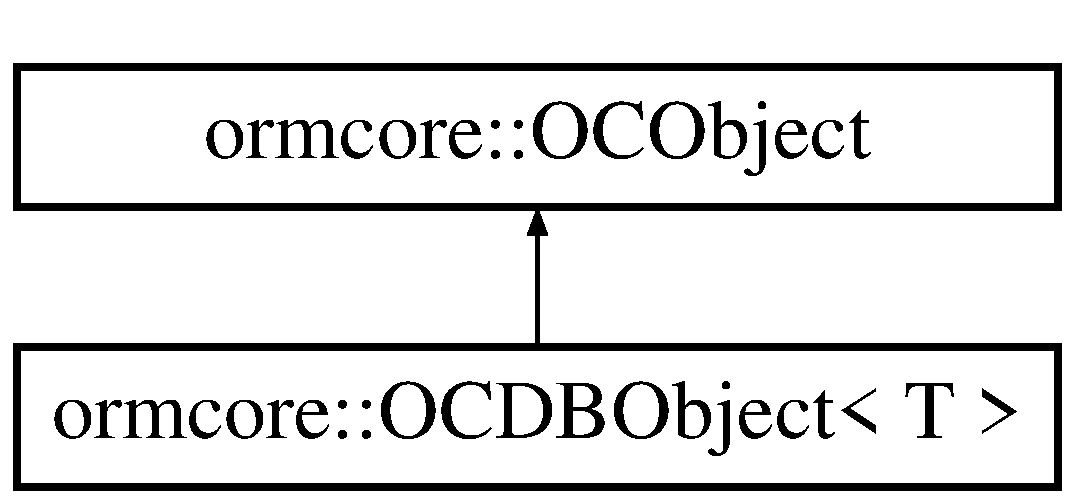
\includegraphics[height=2.000000cm]{classormcore_1_1_o_c_d_b_object}
\end{center}
\end{figure}
\subsection*{\-Public \-Types}
\begin{DoxyCompactItemize}
\item 
enum \{ {\bfseries \-O\-C\-\_\-\-\_\-\-P\-A\-R\-S\-E\-R\-\_\-\-C\-O\-L\-U\-M\-N} =  0, 
{\bfseries \-O\-C\-\_\-\-P\-A\-R\-S\-E\-R\-\_\-\-T\-Y\-P\-E}
 \}
\end{DoxyCompactItemize}
\subsection*{\-Public \-Member \-Functions}
\begin{DoxyCompactItemize}
\item 
\hyperlink{classormcore_1_1_o_c_d_b_object_a46280068ed1abcb08c5f614e787e4dba}{\-O\-C\-D\-B\-Object} ()
\item 
virtual \hyperlink{classormcore_1_1_o_c_d_b_object_a663934fbb05460513439521ef8eadb63}{$\sim$\-O\-C\-D\-B\-Object} ()
\item 
bool \hyperlink{classormcore_1_1_o_c_d_b_object_a7e2e9c0820bc66189a1bcf6efca053d2}{get} (qint64 id)
\item 
void \hyperlink{classormcore_1_1_o_c_d_b_object_a3c51b31ed3af8f9c053f18a8a273629c}{\-Load\-Fields} ()
\item 
quint64 \hyperlink{classormcore_1_1_o_c_d_b_object_a874b6393a9eec12bcca0223498222c19}{id} ()
\item 
void \hyperlink{classormcore_1_1_o_c_d_b_object_abf952a522671d2b77c7098e19854843d}{set\-Id} (quint64 id)
\item 
void \hyperlink{classormcore_1_1_o_c_d_b_object_a8ce6b4690c5fb6f0fba1a8f1d1e2b3fb}{set\-Value} (\-Q\-String field, \-Q\-Variant value)
\item 
\-Q\-Variant \& \hyperlink{classormcore_1_1_o_c_d_b_object_a989b2d6257bf82aaa38f8d15d3d83c2c}{operator\mbox{[}$\,$\mbox{]}} (\-Q\-String key)
\item 
void \hyperlink{classormcore_1_1_o_c_d_b_object_afb6673d0d57d70513847db564915ef78}{save\-If\-Not\-Exists} (\-Q\-String\-List fields=\-Q\-String\-List())
\item 
void \hyperlink{classormcore_1_1_o_c_d_b_object_ac90983398799a3181e145f8057a608ab}{save\-If\-Not\-Exists\-Except} (\-Q\-String\-List exceptions=\-Q\-String\-List())
\item 
void \hyperlink{classormcore_1_1_o_c_d_b_object_adf3f8d09d2cda13348e9834144916e45}{save} ()
\item 
bool \hyperlink{classormcore_1_1_o_c_d_b_object_acb0dd02e72d5714014f7b9856f38db18}{get\-Same\-Values} (\-Q\-String\-List fields=\-Q\-String\-List(), \-Q\-String order\-By=\-Q\-String())
\item 
bool \hyperlink{classormcore_1_1_o_c_d_b_object_a1531bd979b94e095972579a9944734d9}{get\-Same\-Values\-Except} (\-Q\-String\-List fields\-Except=\-Q\-String\-List(), \-Q\-String order\-By=\char`\"{}\char`\"{})
\item 
bool \hyperlink{classormcore_1_1_o_c_d_b_object_a4a508cd7582d12587c81f938eacc7462}{exists\-Same\-Values} (\-Q\-String\-List fields=\-Q\-String\-List())
\item 
bool \hyperlink{classormcore_1_1_o_c_d_b_object_a5a0fbb8f89ed201d2625edd43647207f}{exists\-Same\-Values\-Except} (\-Q\-String\-List fields\-Except=\-Q\-String\-List())
\item 
bool \hyperlink{classormcore_1_1_o_c_d_b_object_ae3f5eb296ca8dfb03ee72fdf1cf5c199}{exists} (\-Q\-String where\-Clause=\char`\"{}\char`\"{})
\end{DoxyCompactItemize}
\subsection*{\-Static \-Public \-Member \-Functions}
\begin{DoxyCompactItemize}
\item 
\hypertarget{classormcore_1_1_o_c_d_b_object_acedb1136e415338d607b7edef6037409}{
static \-Q\-Hash$<$ \-Q\-String, \-Q\-String $>$ {\bfseries parse\-Fields} (\-Q\-String schema)}
\label{classormcore_1_1_o_c_d_b_object_acedb1136e415338d607b7edef6037409}

\item 
static void \hyperlink{classormcore_1_1_o_c_d_b_object_a128132815ade97882e2300743779e46a}{add\-Columns} (\-Q\-Hash$<$ \-Q\-String, \-Q\-String $>$ old\-Fields, \-Q\-Hash$<$ \-Q\-String, \-Q\-String $>$ new\-Fields)
\item 
static void \hyperlink{classormcore_1_1_o_c_d_b_object_a36815ad0bdadcabfdf3ed84e2411e9c1}{recreate\-Table} (\-Q\-Hash$<$ \-Q\-String, \-Q\-String $>$ old\-Fields, \-Q\-Hash$<$ \-Q\-String, \-Q\-String $>$ new\-Fields)
\item 
static void \hyperlink{classormcore_1_1_o_c_d_b_object_a18c394209bf0e80082d884842ea9630a}{create\-Table} ()
\item 
static \-Q\-Hash$<$ \-Q\-String, \-Q\-String $>$ \hyperlink{classormcore_1_1_o_c_d_b_object_ad32aef4a69a116a0fa7ebf7d704d3506}{get\-Table\-Columns} ()
\item 
static void \hyperlink{classormcore_1_1_o_c_d_b_object_a2f72c86621c10110a70ffed11033c38c}{sync\-Database} ()
\item 
static \-Q\-List$<$ \hyperlink{classormcore_1_1_o_c_d_b_object}{\-O\-C\-D\-B\-Object}$<$ \-T $>$ $>$ \hyperlink{classormcore_1_1_o_c_d_b_object_a0617a472caa17e9ca3da70c7386b885c}{objects} (\-Q\-String where\-Clause=\char`\"{}\char`\"{}, \-Q\-String order\-By=\char`\"{}\char`\"{})
\end{DoxyCompactItemize}


\subsection{\-Detailed \-Description}
\subsubsection*{template$<$class \-T$>$class ormcore\-::\-O\-C\-D\-B\-Object$<$ T $>$}

\-Template base dos objetos do banco de dados. 

\subsection{\-Constructor \& \-Destructor \-Documentation}
\hypertarget{classormcore_1_1_o_c_d_b_object_a46280068ed1abcb08c5f614e787e4dba}{
\index{ormcore\-::\-O\-C\-D\-B\-Object@{ormcore\-::\-O\-C\-D\-B\-Object}!\-O\-C\-D\-B\-Object@{\-O\-C\-D\-B\-Object}}
\index{\-O\-C\-D\-B\-Object@{\-O\-C\-D\-B\-Object}!ormcore::OCDBObject@{ormcore\-::\-O\-C\-D\-B\-Object}}
\subsubsection[{\-O\-C\-D\-B\-Object}]{\setlength{\rightskip}{0pt plus 5cm}template$<$class \-T$>$ {\bf ormcore\-::\-O\-C\-D\-B\-Object}$<$ \-T $>$\-::{\bf \-O\-C\-D\-B\-Object} (
\begin{DoxyParamCaption}
{}
\end{DoxyParamCaption}
)\hspace{0.3cm}{\ttfamily  \mbox{[}inline\mbox{]}}}}
\label{classormcore_1_1_o_c_d_b_object_a46280068ed1abcb08c5f614e787e4dba}
\-Construtor da classe \-Testa se o objeto passado para o template é o correto (precisa herdar de \hyperlink{classormcore_1_1_o_c_model}{\-O\-C\-Model}). \begin{DoxySeeAlso}{\-See also}
\hyperlink{classormcore_1_1_o_c_model}{\-O\-C\-Model} 
\end{DoxySeeAlso}
\hypertarget{classormcore_1_1_o_c_d_b_object_a663934fbb05460513439521ef8eadb63}{
\index{ormcore\-::\-O\-C\-D\-B\-Object@{ormcore\-::\-O\-C\-D\-B\-Object}!$\sim$\-O\-C\-D\-B\-Object@{$\sim$\-O\-C\-D\-B\-Object}}
\index{$\sim$\-O\-C\-D\-B\-Object@{$\sim$\-O\-C\-D\-B\-Object}!ormcore::OCDBObject@{ormcore\-::\-O\-C\-D\-B\-Object}}
\subsubsection[{$\sim$\-O\-C\-D\-B\-Object}]{\setlength{\rightskip}{0pt plus 5cm}template$<$class \-T$>$ virtual {\bf ormcore\-::\-O\-C\-D\-B\-Object}$<$ \-T $>$\-::$\sim${\bf \-O\-C\-D\-B\-Object} (
\begin{DoxyParamCaption}
{}
\end{DoxyParamCaption}
)\hspace{0.3cm}{\ttfamily  \mbox{[}inline, virtual\mbox{]}}}}
\label{classormcore_1_1_o_c_d_b_object_a663934fbb05460513439521ef8eadb63}
\-Destrutor da classe 

\subsection{\-Member \-Function \-Documentation}
\hypertarget{classormcore_1_1_o_c_d_b_object_a128132815ade97882e2300743779e46a}{
\index{ormcore\-::\-O\-C\-D\-B\-Object@{ormcore\-::\-O\-C\-D\-B\-Object}!add\-Columns@{add\-Columns}}
\index{add\-Columns@{add\-Columns}!ormcore::OCDBObject@{ormcore\-::\-O\-C\-D\-B\-Object}}
\subsubsection[{add\-Columns}]{\setlength{\rightskip}{0pt plus 5cm}template$<$class \-T$>$ static void {\bf ormcore\-::\-O\-C\-D\-B\-Object}$<$ \-T $>$\-::add\-Columns (
\begin{DoxyParamCaption}
\item[{\-Q\-Hash$<$ \-Q\-String, \-Q\-String $>$}]{old\-Fields, }
\item[{\-Q\-Hash$<$ \-Q\-String, \-Q\-String $>$}]{new\-Fields}
\end{DoxyParamCaption}
)\hspace{0.3cm}{\ttfamily  \mbox{[}inline, static\mbox{]}}}}
\label{classormcore_1_1_o_c_d_b_object_a128132815ade97882e2300743779e46a}
\-Adiciona colunas à tabela 
\begin{DoxyParams}{\-Parameters}
{\em old\-Fields} & \-Campos da tabela antiga \\
\hline
{\em new\-Fields} & \-Campos da tabela nova \\
\hline
\end{DoxyParams}

\begin{DoxyExceptions}{\-Exceptions}
{\em \hyperlink{classormcore_1_1_o_c_s_q_l_exception}{\-O\-C\-S\-Q\-L\-Exception}} & \\
\hline
\end{DoxyExceptions}
\hypertarget{classormcore_1_1_o_c_d_b_object_a18c394209bf0e80082d884842ea9630a}{
\index{ormcore\-::\-O\-C\-D\-B\-Object@{ormcore\-::\-O\-C\-D\-B\-Object}!create\-Table@{create\-Table}}
\index{create\-Table@{create\-Table}!ormcore::OCDBObject@{ormcore\-::\-O\-C\-D\-B\-Object}}
\subsubsection[{create\-Table}]{\setlength{\rightskip}{0pt plus 5cm}template$<$class \-T$>$ static void {\bf ormcore\-::\-O\-C\-D\-B\-Object}$<$ \-T $>$\-::create\-Table (
\begin{DoxyParamCaption}
{}
\end{DoxyParamCaption}
)\hspace{0.3cm}{\ttfamily  \mbox{[}inline, static\mbox{]}}}}
\label{classormcore_1_1_o_c_d_b_object_a18c394209bf0e80082d884842ea9630a}
\-Criar tabela no banco de dados 
\begin{DoxyExceptions}{\-Exceptions}
{\em \hyperlink{classormcore_1_1_o_c_s_q_l_exception}{\-O\-C\-S\-Q\-L\-Exception}} & \\
\hline
\end{DoxyExceptions}
\hypertarget{classormcore_1_1_o_c_d_b_object_ae3f5eb296ca8dfb03ee72fdf1cf5c199}{
\index{ormcore\-::\-O\-C\-D\-B\-Object@{ormcore\-::\-O\-C\-D\-B\-Object}!exists@{exists}}
\index{exists@{exists}!ormcore::OCDBObject@{ormcore\-::\-O\-C\-D\-B\-Object}}
\subsubsection[{exists}]{\setlength{\rightskip}{0pt plus 5cm}template$<$class \-T$>$ bool {\bf ormcore\-::\-O\-C\-D\-B\-Object}$<$ \-T $>$\-::exists (
\begin{DoxyParamCaption}
\item[{\-Q\-String}]{where\-Clause = {\ttfamily \char`\"{}\char`\"{}}}
\end{DoxyParamCaption}
)\hspace{0.3cm}{\ttfamily  \mbox{[}inline\mbox{]}}}}
\label{classormcore_1_1_o_c_d_b_object_ae3f5eb296ca8dfb03ee72fdf1cf5c199}
\-Verifica se existe o valor no banco de dados com a where\-Clause informada como parâmetro. 
\begin{DoxyParams}{\-Parameters}
{\em where\-Clause} & \-Clausula where no banco de dados sem o \char`\"{}\-W\-H\-E\-R\-E\char`\"{} \\
\hline
\end{DoxyParams}
\begin{DoxyReturn}{\-Returns}
\-Verdadeiro caso exista, ou falso em caso negativo 
\end{DoxyReturn}
\hypertarget{classormcore_1_1_o_c_d_b_object_a4a508cd7582d12587c81f938eacc7462}{
\index{ormcore\-::\-O\-C\-D\-B\-Object@{ormcore\-::\-O\-C\-D\-B\-Object}!exists\-Same\-Values@{exists\-Same\-Values}}
\index{exists\-Same\-Values@{exists\-Same\-Values}!ormcore::OCDBObject@{ormcore\-::\-O\-C\-D\-B\-Object}}
\subsubsection[{exists\-Same\-Values}]{\setlength{\rightskip}{0pt plus 5cm}template$<$class \-T$>$ bool {\bf ormcore\-::\-O\-C\-D\-B\-Object}$<$ \-T $>$\-::exists\-Same\-Values (
\begin{DoxyParamCaption}
\item[{\-Q\-String\-List}]{fields = {\ttfamily \-Q\-String\-List()}}
\end{DoxyParamCaption}
)\hspace{0.3cm}{\ttfamily  \mbox{[}inline\mbox{]}}}}
\label{classormcore_1_1_o_c_d_b_object_a4a508cd7582d12587c81f938eacc7462}
\-Verifica se existe já um registro no banco de dados com os mesmos valores (\-Exceto id, que pode ser diferente) e exceto campos passados como parâmetro 
\begin{DoxyParams}{\-Parameters}
{\em fields\-Except} & \-Campos para ignorar na comparação \\
\hline
\end{DoxyParams}
\begin{DoxyReturn}{\-Returns}
\-Retorna verdadeiro caso já exista o registro, ou falso em caso negativo 
\end{DoxyReturn}
\hypertarget{classormcore_1_1_o_c_d_b_object_a5a0fbb8f89ed201d2625edd43647207f}{
\index{ormcore\-::\-O\-C\-D\-B\-Object@{ormcore\-::\-O\-C\-D\-B\-Object}!exists\-Same\-Values\-Except@{exists\-Same\-Values\-Except}}
\index{exists\-Same\-Values\-Except@{exists\-Same\-Values\-Except}!ormcore::OCDBObject@{ormcore\-::\-O\-C\-D\-B\-Object}}
\subsubsection[{exists\-Same\-Values\-Except}]{\setlength{\rightskip}{0pt plus 5cm}template$<$class \-T$>$ bool {\bf ormcore\-::\-O\-C\-D\-B\-Object}$<$ \-T $>$\-::exists\-Same\-Values\-Except (
\begin{DoxyParamCaption}
\item[{\-Q\-String\-List}]{fields\-Except = {\ttfamily \-Q\-String\-List()}}
\end{DoxyParamCaption}
)\hspace{0.3cm}{\ttfamily  \mbox{[}inline\mbox{]}}}}
\label{classormcore_1_1_o_c_d_b_object_a5a0fbb8f89ed201d2625edd43647207f}
\-Verifica se existe já um registro no banco de dados com os mesmos valores (\-Exceto id, que pode ser diferente) e exceto campos passados como parâmetro 
\begin{DoxyParams}{\-Parameters}
{\em fields\-Except} & \-Campos para ignorar na comparação \\
\hline
\end{DoxyParams}
\begin{DoxyReturn}{\-Returns}
\-Retorna verdadeiro caso já exista o registro, ou falso em caso negativo 
\end{DoxyReturn}
\hypertarget{classormcore_1_1_o_c_d_b_object_a7e2e9c0820bc66189a1bcf6efca053d2}{
\index{ormcore\-::\-O\-C\-D\-B\-Object@{ormcore\-::\-O\-C\-D\-B\-Object}!get@{get}}
\index{get@{get}!ormcore::OCDBObject@{ormcore\-::\-O\-C\-D\-B\-Object}}
\subsubsection[{get}]{\setlength{\rightskip}{0pt plus 5cm}template$<$class \-T$>$ bool {\bf ormcore\-::\-O\-C\-D\-B\-Object}$<$ \-T $>$\-::get (
\begin{DoxyParamCaption}
\item[{qint64}]{id}
\end{DoxyParamCaption}
)\hspace{0.3cm}{\ttfamily  \mbox{[}inline\mbox{]}}}}
\label{classormcore_1_1_o_c_d_b_object_a7e2e9c0820bc66189a1bcf6efca053d2}
\-Carrega o objeto do banco do dados com base no id passado como parâmetro. 
\begin{DoxyExceptions}{\-Exceptions}
{\em \hyperlink{classormcore_1_1_o_c_s_q_l_exception}{\-O\-C\-S\-Q\-L\-Exception}} & \\
\hline
\end{DoxyExceptions}

\begin{DoxyParams}{\-Parameters}
{\em id} & \-Identificador do objeto no banco de dados. \\
\hline
\end{DoxyParams}
\begin{DoxyReturn}{\-Returns}
\-Valor booleano indicando se o objeto foi carregado ou não. 
\end{DoxyReturn}
\hypertarget{classormcore_1_1_o_c_d_b_object_acb0dd02e72d5714014f7b9856f38db18}{
\index{ormcore\-::\-O\-C\-D\-B\-Object@{ormcore\-::\-O\-C\-D\-B\-Object}!get\-Same\-Values@{get\-Same\-Values}}
\index{get\-Same\-Values@{get\-Same\-Values}!ormcore::OCDBObject@{ormcore\-::\-O\-C\-D\-B\-Object}}
\subsubsection[{get\-Same\-Values}]{\setlength{\rightskip}{0pt plus 5cm}template$<$class \-T$>$ bool {\bf ormcore\-::\-O\-C\-D\-B\-Object}$<$ \-T $>$\-::get\-Same\-Values (
\begin{DoxyParamCaption}
\item[{\-Q\-String\-List}]{fields = {\ttfamily \-Q\-String\-List()}, }
\item[{\-Q\-String}]{order\-By = {\ttfamily \-Q\-String()}}
\end{DoxyParamCaption}
)\hspace{0.3cm}{\ttfamily  \mbox{[}inline\mbox{]}}}}
\label{classormcore_1_1_o_c_d_b_object_acb0dd02e72d5714014f7b9856f38db18}
\-Verifica se existe já um registro no banco de dados com os mesmos valores do objeto, com os campos passados como parâmetro e carrega o primeiro valor encontrado 
\begin{DoxyParams}{\-Parameters}
{\em fields} & \-Campos para comparar \\
\hline
\end{DoxyParams}
\begin{DoxyReturn}{\-Returns}
\-Retorna verdadeiro caso já exista o registro e tenha sido carregado, ou falso em caso negativo 
\end{DoxyReturn}
\hypertarget{classormcore_1_1_o_c_d_b_object_a1531bd979b94e095972579a9944734d9}{
\index{ormcore\-::\-O\-C\-D\-B\-Object@{ormcore\-::\-O\-C\-D\-B\-Object}!get\-Same\-Values\-Except@{get\-Same\-Values\-Except}}
\index{get\-Same\-Values\-Except@{get\-Same\-Values\-Except}!ormcore::OCDBObject@{ormcore\-::\-O\-C\-D\-B\-Object}}
\subsubsection[{get\-Same\-Values\-Except}]{\setlength{\rightskip}{0pt plus 5cm}template$<$class \-T$>$ bool {\bf ormcore\-::\-O\-C\-D\-B\-Object}$<$ \-T $>$\-::get\-Same\-Values\-Except (
\begin{DoxyParamCaption}
\item[{\-Q\-String\-List}]{fields\-Except = {\ttfamily \-Q\-String\-List()}, }
\item[{\-Q\-String}]{order\-By = {\ttfamily \char`\"{}\char`\"{}}}
\end{DoxyParamCaption}
)\hspace{0.3cm}{\ttfamily  \mbox{[}inline\mbox{]}}}}
\label{classormcore_1_1_o_c_d_b_object_a1531bd979b94e095972579a9944734d9}
\-Verifica se existe já um registro no banco de dados com os mesmos valores (\-Exceto id, que pode ser diferente) e exceto campos passados como parâmetro e carrega o primeiro valor encontrado 
\begin{DoxyParams}{\-Parameters}
{\em fields\-Except} & \-Campos para ignorar na comparação \\
\hline
\end{DoxyParams}
\begin{DoxyReturn}{\-Returns}
\-Retorna verdadeiro caso já exista o registro e tenha sido carregado, ou falso em caso negativo 
\end{DoxyReturn}
\hypertarget{classormcore_1_1_o_c_d_b_object_ad32aef4a69a116a0fa7ebf7d704d3506}{
\index{ormcore\-::\-O\-C\-D\-B\-Object@{ormcore\-::\-O\-C\-D\-B\-Object}!get\-Table\-Columns@{get\-Table\-Columns}}
\index{get\-Table\-Columns@{get\-Table\-Columns}!ormcore::OCDBObject@{ormcore\-::\-O\-C\-D\-B\-Object}}
\subsubsection[{get\-Table\-Columns}]{\setlength{\rightskip}{0pt plus 5cm}template$<$class \-T$>$ static \-Q\-Hash$<$\-Q\-String, \-Q\-String$>$ {\bf ormcore\-::\-O\-C\-D\-B\-Object}$<$ \-T $>$\-::get\-Table\-Columns (
\begin{DoxyParamCaption}
{}
\end{DoxyParamCaption}
)\hspace{0.3cm}{\ttfamily  \mbox{[}inline, static\mbox{]}}}}
\label{classormcore_1_1_o_c_d_b_object_ad32aef4a69a116a0fa7ebf7d704d3506}
\-Retornar nomes das colunas do banco de dados \begin{DoxyReturn}{\-Returns}
nomes das colunas em uma \-Q\-Hash 
\end{DoxyReturn}

\begin{DoxyExceptions}{\-Exceptions}
{\em \hyperlink{classormcore_1_1_o_c_s_q_l_exception}{\-O\-C\-S\-Q\-L\-Exception}} & \\
\hline
\end{DoxyExceptions}
\hypertarget{classormcore_1_1_o_c_d_b_object_a874b6393a9eec12bcca0223498222c19}{
\index{ormcore\-::\-O\-C\-D\-B\-Object@{ormcore\-::\-O\-C\-D\-B\-Object}!id@{id}}
\index{id@{id}!ormcore::OCDBObject@{ormcore\-::\-O\-C\-D\-B\-Object}}
\subsubsection[{id}]{\setlength{\rightskip}{0pt plus 5cm}template$<$class \-T$>$ quint64 {\bf ormcore\-::\-O\-C\-D\-B\-Object}$<$ \-T $>$\-::id (
\begin{DoxyParamCaption}
{}
\end{DoxyParamCaption}
)\hspace{0.3cm}{\ttfamily  \mbox{[}inline\mbox{]}}}}
\label{classormcore_1_1_o_c_d_b_object_a874b6393a9eec12bcca0223498222c19}
\-Retorna o id do objeto \begin{DoxyReturn}{\-Returns}
id do objeto 
\end{DoxyReturn}
\hypertarget{classormcore_1_1_o_c_d_b_object_a3c51b31ed3af8f9c053f18a8a273629c}{
\index{ormcore\-::\-O\-C\-D\-B\-Object@{ormcore\-::\-O\-C\-D\-B\-Object}!\-Load\-Fields@{\-Load\-Fields}}
\index{\-Load\-Fields@{\-Load\-Fields}!ormcore::OCDBObject@{ormcore\-::\-O\-C\-D\-B\-Object}}
\subsubsection[{\-Load\-Fields}]{\setlength{\rightskip}{0pt plus 5cm}template$<$class \-T$>$ void {\bf ormcore\-::\-O\-C\-D\-B\-Object}$<$ \-T $>$\-::\-Load\-Fields (
\begin{DoxyParamCaption}
{}
\end{DoxyParamCaption}
)\hspace{0.3cm}{\ttfamily  \mbox{[}inline\mbox{]}}}}
\label{classormcore_1_1_o_c_d_b_object_a3c51b31ed3af8f9c053f18a8a273629c}
\-Carrega campos baseado no schema \hypertarget{classormcore_1_1_o_c_d_b_object_a0617a472caa17e9ca3da70c7386b885c}{
\index{ormcore\-::\-O\-C\-D\-B\-Object@{ormcore\-::\-O\-C\-D\-B\-Object}!objects@{objects}}
\index{objects@{objects}!ormcore::OCDBObject@{ormcore\-::\-O\-C\-D\-B\-Object}}
\subsubsection[{objects}]{\setlength{\rightskip}{0pt plus 5cm}template$<$class \-T$>$ static \-Q\-List$<$ {\bf \-O\-C\-D\-B\-Object}$<$\-T$>$ $>$ {\bf ormcore\-::\-O\-C\-D\-B\-Object}$<$ \-T $>$\-::objects (
\begin{DoxyParamCaption}
\item[{\-Q\-String}]{where\-Clause = {\ttfamily \char`\"{}\char`\"{}}, }
\item[{\-Q\-String}]{order\-By = {\ttfamily \char`\"{}\char`\"{}}}
\end{DoxyParamCaption}
)\hspace{0.3cm}{\ttfamily  \mbox{[}inline, static\mbox{]}}}}
\label{classormcore_1_1_o_c_d_b_object_a0617a472caa17e9ca3da70c7386b885c}
\-Filtra dados da base de dados com base nos paramêtros 
\begin{DoxyParams}{\-Parameters}
{\em where\-Clause} & \-Clausula where no banco de dados sem o \char`\"{}\-W\-H\-E\-R\-E\char`\"{} \\
\hline
\end{DoxyParams}
\begin{DoxyReturn}{\-Returns}
\-Lista de objetos retornados do banco de dados 
\end{DoxyReturn}

\begin{DoxyExceptions}{\-Exceptions}
{\em \hyperlink{classormcore_1_1_o_c_s_q_l_exception}{\-O\-C\-S\-Q\-L\-Exception}} & \\
\hline
\end{DoxyExceptions}
\hypertarget{classormcore_1_1_o_c_d_b_object_a989b2d6257bf82aaa38f8d15d3d83c2c}{
\index{ormcore\-::\-O\-C\-D\-B\-Object@{ormcore\-::\-O\-C\-D\-B\-Object}!operator\mbox{[}$\,$\mbox{]}@{operator[]}}
\index{operator\mbox{[}$\,$\mbox{]}@{operator[]}!ormcore::OCDBObject@{ormcore\-::\-O\-C\-D\-B\-Object}}
\subsubsection[{operator[]}]{\setlength{\rightskip}{0pt plus 5cm}template$<$class \-T$>$ \-Q\-Variant\& {\bf ormcore\-::\-O\-C\-D\-B\-Object}$<$ \-T $>$\-::operator\mbox{[}$\,$\mbox{]} (
\begin{DoxyParamCaption}
\item[{\-Q\-String}]{key}
\end{DoxyParamCaption}
)\hspace{0.3cm}{\ttfamily  \mbox{[}inline\mbox{]}}}}
\label{classormcore_1_1_o_c_d_b_object_a989b2d6257bf82aaa38f8d15d3d83c2c}
\-Sobrecarga do operador \mbox{[}\mbox{]} para atribuir ou recuperar o valor de um campo do objeto \-Mantendo uma equivalencia com o nome do campo na base de dados. 
\begin{DoxyParams}{\-Parameters}
{\em key} & \-Nome do campo na base de dados \\
\hline
\end{DoxyParams}
\begin{DoxyReturn}{\-Returns}
\-O valor armazenado pelo campo 
\end{DoxyReturn}
\hypertarget{classormcore_1_1_o_c_d_b_object_a36815ad0bdadcabfdf3ed84e2411e9c1}{
\index{ormcore\-::\-O\-C\-D\-B\-Object@{ormcore\-::\-O\-C\-D\-B\-Object}!recreate\-Table@{recreate\-Table}}
\index{recreate\-Table@{recreate\-Table}!ormcore::OCDBObject@{ormcore\-::\-O\-C\-D\-B\-Object}}
\subsubsection[{recreate\-Table}]{\setlength{\rightskip}{0pt plus 5cm}template$<$class \-T$>$ static void {\bf ormcore\-::\-O\-C\-D\-B\-Object}$<$ \-T $>$\-::recreate\-Table (
\begin{DoxyParamCaption}
\item[{\-Q\-Hash$<$ \-Q\-String, \-Q\-String $>$}]{old\-Fields, }
\item[{\-Q\-Hash$<$ \-Q\-String, \-Q\-String $>$}]{new\-Fields}
\end{DoxyParamCaption}
)\hspace{0.3cm}{\ttfamily  \mbox{[}inline, static\mbox{]}}}}
\label{classormcore_1_1_o_c_d_b_object_a36815ad0bdadcabfdf3ed84e2411e9c1}
\-Recria tabela para remover campos 
\begin{DoxyParams}{\-Parameters}
{\em old\-Fields} & \-Campos da tabela antiga \\
\hline
{\em new\-Fields} & \-Campos da tabela nova \\
\hline
\end{DoxyParams}

\begin{DoxyExceptions}{\-Exceptions}
{\em \hyperlink{classormcore_1_1_o_c_s_q_l_exception}{\-O\-C\-S\-Q\-L\-Exception}} & \\
\hline
\end{DoxyExceptions}
\hypertarget{classormcore_1_1_o_c_d_b_object_adf3f8d09d2cda13348e9834144916e45}{
\index{ormcore\-::\-O\-C\-D\-B\-Object@{ormcore\-::\-O\-C\-D\-B\-Object}!save@{save}}
\index{save@{save}!ormcore::OCDBObject@{ormcore\-::\-O\-C\-D\-B\-Object}}
\subsubsection[{save}]{\setlength{\rightskip}{0pt plus 5cm}template$<$class \-T$>$ void {\bf ormcore\-::\-O\-C\-D\-B\-Object}$<$ \-T $>$\-::save (
\begin{DoxyParamCaption}
{}
\end{DoxyParamCaption}
)\hspace{0.3cm}{\ttfamily  \mbox{[}inline\mbox{]}}}}
\label{classormcore_1_1_o_c_d_b_object_adf3f8d09d2cda13348e9834144916e45}
\-Salva as alterações na base de dados, caso o registro ainda não exista então é feita uma inserção dos dados na base. 
\begin{DoxyExceptions}{\-Exceptions}
{\em \hyperlink{classormcore_1_1_o_c_s_q_l_exception}{\-O\-C\-S\-Q\-L\-Exception}} & \\
\hline
\end{DoxyExceptions}
\hypertarget{classormcore_1_1_o_c_d_b_object_afb6673d0d57d70513847db564915ef78}{
\index{ormcore\-::\-O\-C\-D\-B\-Object@{ormcore\-::\-O\-C\-D\-B\-Object}!save\-If\-Not\-Exists@{save\-If\-Not\-Exists}}
\index{save\-If\-Not\-Exists@{save\-If\-Not\-Exists}!ormcore::OCDBObject@{ormcore\-::\-O\-C\-D\-B\-Object}}
\subsubsection[{save\-If\-Not\-Exists}]{\setlength{\rightskip}{0pt plus 5cm}template$<$class \-T$>$ void {\bf ormcore\-::\-O\-C\-D\-B\-Object}$<$ \-T $>$\-::save\-If\-Not\-Exists (
\begin{DoxyParamCaption}
\item[{\-Q\-String\-List}]{fields = {\ttfamily \-Q\-String\-List()}}
\end{DoxyParamCaption}
)\hspace{0.3cm}{\ttfamily  \mbox{[}inline\mbox{]}}}}
\label{classormcore_1_1_o_c_d_b_object_afb6673d0d57d70513847db564915ef78}
\-Salva registro apenas se já não existe na base de dados. 
\begin{DoxyParams}{\-Parameters}
{\em fields} & \-Campos para comparar quando verificar se já existe \\
\hline
\end{DoxyParams}
\hypertarget{classormcore_1_1_o_c_d_b_object_ac90983398799a3181e145f8057a608ab}{
\index{ormcore\-::\-O\-C\-D\-B\-Object@{ormcore\-::\-O\-C\-D\-B\-Object}!save\-If\-Not\-Exists\-Except@{save\-If\-Not\-Exists\-Except}}
\index{save\-If\-Not\-Exists\-Except@{save\-If\-Not\-Exists\-Except}!ormcore::OCDBObject@{ormcore\-::\-O\-C\-D\-B\-Object}}
\subsubsection[{save\-If\-Not\-Exists\-Except}]{\setlength{\rightskip}{0pt plus 5cm}template$<$class \-T$>$ void {\bf ormcore\-::\-O\-C\-D\-B\-Object}$<$ \-T $>$\-::save\-If\-Not\-Exists\-Except (
\begin{DoxyParamCaption}
\item[{\-Q\-String\-List}]{exceptions = {\ttfamily \-Q\-String\-List()}}
\end{DoxyParamCaption}
)\hspace{0.3cm}{\ttfamily  \mbox{[}inline\mbox{]}}}}
\label{classormcore_1_1_o_c_d_b_object_ac90983398799a3181e145f8057a608ab}
\-Salva registro apenas se já não existe na base de dados. 
\begin{DoxyParams}{\-Parameters}
{\em exeptions} & \-Campos para não comparar quando verificar se já existe \\
\hline
\end{DoxyParams}
\hypertarget{classormcore_1_1_o_c_d_b_object_abf952a522671d2b77c7098e19854843d}{
\index{ormcore\-::\-O\-C\-D\-B\-Object@{ormcore\-::\-O\-C\-D\-B\-Object}!set\-Id@{set\-Id}}
\index{set\-Id@{set\-Id}!ormcore::OCDBObject@{ormcore\-::\-O\-C\-D\-B\-Object}}
\subsubsection[{set\-Id}]{\setlength{\rightskip}{0pt plus 5cm}template$<$class \-T$>$ void {\bf ormcore\-::\-O\-C\-D\-B\-Object}$<$ \-T $>$\-::set\-Id (
\begin{DoxyParamCaption}
\item[{quint64}]{id}
\end{DoxyParamCaption}
)\hspace{0.3cm}{\ttfamily  \mbox{[}inline\mbox{]}}}}
\label{classormcore_1_1_o_c_d_b_object_abf952a522671d2b77c7098e19854843d}
\-Atribui o valor do id do objeto 
\begin{DoxyParams}{\-Parameters}
{\em id} & do objeto \\
\hline
\end{DoxyParams}
\hypertarget{classormcore_1_1_o_c_d_b_object_a8ce6b4690c5fb6f0fba1a8f1d1e2b3fb}{
\index{ormcore\-::\-O\-C\-D\-B\-Object@{ormcore\-::\-O\-C\-D\-B\-Object}!set\-Value@{set\-Value}}
\index{set\-Value@{set\-Value}!ormcore::OCDBObject@{ormcore\-::\-O\-C\-D\-B\-Object}}
\subsubsection[{set\-Value}]{\setlength{\rightskip}{0pt plus 5cm}template$<$class \-T$>$ void {\bf ormcore\-::\-O\-C\-D\-B\-Object}$<$ \-T $>$\-::set\-Value (
\begin{DoxyParamCaption}
\item[{\-Q\-String}]{field, }
\item[{\-Q\-Variant}]{value}
\end{DoxyParamCaption}
)\hspace{0.3cm}{\ttfamily  \mbox{[}inline\mbox{]}}}}
\label{classormcore_1_1_o_c_d_b_object_a8ce6b4690c5fb6f0fba1a8f1d1e2b3fb}
\-Atribui o valor value para o campo field do objeto 
\begin{DoxyParams}{\-Parameters}
{\em field} & \-Campo do objeto ao qual será atribuído o novo valor \\
\hline
{\em value} & \-Novo valor a ser assinalado para o campo field \\
\hline
\end{DoxyParams}
\hypertarget{classormcore_1_1_o_c_d_b_object_a2f72c86621c10110a70ffed11033c38c}{
\index{ormcore\-::\-O\-C\-D\-B\-Object@{ormcore\-::\-O\-C\-D\-B\-Object}!sync\-Database@{sync\-Database}}
\index{sync\-Database@{sync\-Database}!ormcore::OCDBObject@{ormcore\-::\-O\-C\-D\-B\-Object}}
\subsubsection[{sync\-Database}]{\setlength{\rightskip}{0pt plus 5cm}template$<$class \-T$>$ static void {\bf ormcore\-::\-O\-C\-D\-B\-Object}$<$ \-T $>$\-::sync\-Database (
\begin{DoxyParamCaption}
{}
\end{DoxyParamCaption}
)\hspace{0.3cm}{\ttfamily  \mbox{[}inline, static\mbox{]}}}}
\label{classormcore_1_1_o_c_d_b_object_a2f72c86621c10110a70ffed11033c38c}
\-Sincroniza a base de dados, ou seja, cria a tabela equivalente ao modelo, caso ela não exista. 
\begin{DoxyExceptions}{\-Exceptions}
{\em \hyperlink{classormcore_1_1_o_c_s_q_l_exception}{\-O\-C\-S\-Q\-L\-Exception}} & \\
\hline
\end{DoxyExceptions}


\-The documentation for this class was generated from the following file\-:\begin{DoxyCompactItemize}
\item 
\-O\-R\-M\-C++/include/ocdbobject.\-h\end{DoxyCompactItemize}

\hypertarget{classormcore_1_1_o_c_exception}{
\section{ormcore\-:\-:\-O\-C\-Exception \-Class \-Reference}
\label{classormcore_1_1_o_c_exception}\index{ormcore\-::\-O\-C\-Exception@{ormcore\-::\-O\-C\-Exception}}
}


{\ttfamily \#include $<$ocexception.\-h$>$}

\-Inheritance diagram for ormcore\-:\-:\-O\-C\-Exception\-:\begin{figure}[H]
\begin{center}
\leavevmode
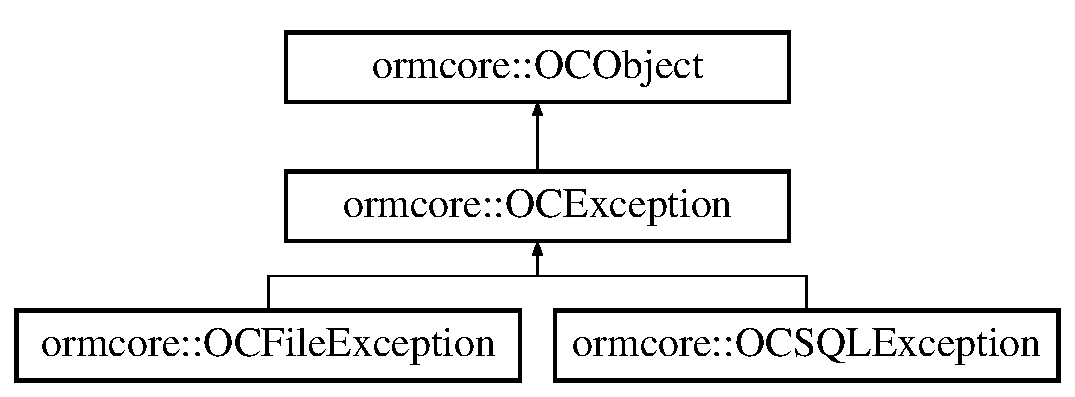
\includegraphics[height=3.000000cm]{classormcore_1_1_o_c_exception}
\end{center}
\end{figure}
\subsection*{\-Public \-Member \-Functions}
\begin{DoxyCompactItemize}
\item 
\hyperlink{classormcore_1_1_o_c_exception_a6440881bb50cce3cbb632ec1495fb9aa}{\-O\-C\-Exception} (\-Q\-String file\-Name, \-Q\-String method\-Name, \-Q\-String message, quint32 line\-No)
\item 
\-Q\-String \hyperlink{classormcore_1_1_o_c_exception_afcdc3ba4ec06269e610baee1210ad2ee}{file\-Name} ()
\item 
\-Q\-String \hyperlink{classormcore_1_1_o_c_exception_a94319bc7771c56ab6797a9e4bdd0dab9}{method\-Name} ()
\item 
\-Q\-String \hyperlink{classormcore_1_1_o_c_exception_a2e21a17f2e298904f50f9f5703378515}{message} ()
\item 
quint32 \hyperlink{classormcore_1_1_o_c_exception_a4df01cf9ef5d6c3b704f4e1486163120}{line\-No} ()
\end{DoxyCompactItemize}


\subsection{\-Detailed \-Description}
\-Classe base das excessões 

\subsection{\-Constructor \& \-Destructor \-Documentation}
\hypertarget{classormcore_1_1_o_c_exception_a6440881bb50cce3cbb632ec1495fb9aa}{
\index{ormcore\-::\-O\-C\-Exception@{ormcore\-::\-O\-C\-Exception}!\-O\-C\-Exception@{\-O\-C\-Exception}}
\index{\-O\-C\-Exception@{\-O\-C\-Exception}!ormcore::OCException@{ormcore\-::\-O\-C\-Exception}}
\subsubsection[{\-O\-C\-Exception}]{\setlength{\rightskip}{0pt plus 5cm}ormcore\-::\-O\-C\-Exception\-::\-O\-C\-Exception (
\begin{DoxyParamCaption}
\item[{\-Q\-String}]{file\-Name, }
\item[{\-Q\-String}]{method\-Name, }
\item[{\-Q\-String}]{message, }
\item[{quint32}]{line\-No}
\end{DoxyParamCaption}
)\hspace{0.3cm}{\ttfamily  \mbox{[}inline\mbox{]}}}}
\label{classormcore_1_1_o_c_exception_a6440881bb50cce3cbb632ec1495fb9aa}
\-Construtor da classe, com os seguintes parâmetros\-: 
\begin{DoxyParams}{\-Parameters}
{\em file\-Name} & \-Nome do arquivo onde foi gerada a excessão \\
\hline
{\em method\-Name} & \-Nome do método onde foi gerada a excessão \\
\hline
{\em message} & \-Mensagem da excessão gerada \\
\hline
{\em line\-No} & \-Número da linha no arquivo onde foi gerada a excessão \\
\hline
\end{DoxyParams}


\subsection{\-Member \-Function \-Documentation}
\hypertarget{classormcore_1_1_o_c_exception_afcdc3ba4ec06269e610baee1210ad2ee}{
\index{ormcore\-::\-O\-C\-Exception@{ormcore\-::\-O\-C\-Exception}!file\-Name@{file\-Name}}
\index{file\-Name@{file\-Name}!ormcore::OCException@{ormcore\-::\-O\-C\-Exception}}
\subsubsection[{file\-Name}]{\setlength{\rightskip}{0pt plus 5cm}\-Q\-String ormcore\-::\-O\-C\-Exception\-::file\-Name (
\begin{DoxyParamCaption}
{}
\end{DoxyParamCaption}
)\hspace{0.3cm}{\ttfamily  \mbox{[}inline\mbox{]}}}}
\label{classormcore_1_1_o_c_exception_afcdc3ba4ec06269e610baee1210ad2ee}
\begin{DoxyReturn}{\-Returns}
\-Nome do arquivo onde foi gerada a excessão 
\end{DoxyReturn}
\hypertarget{classormcore_1_1_o_c_exception_a4df01cf9ef5d6c3b704f4e1486163120}{
\index{ormcore\-::\-O\-C\-Exception@{ormcore\-::\-O\-C\-Exception}!line\-No@{line\-No}}
\index{line\-No@{line\-No}!ormcore::OCException@{ormcore\-::\-O\-C\-Exception}}
\subsubsection[{line\-No}]{\setlength{\rightskip}{0pt plus 5cm}quint32 ormcore\-::\-O\-C\-Exception\-::line\-No (
\begin{DoxyParamCaption}
{}
\end{DoxyParamCaption}
)\hspace{0.3cm}{\ttfamily  \mbox{[}inline\mbox{]}}}}
\label{classormcore_1_1_o_c_exception_a4df01cf9ef5d6c3b704f4e1486163120}
\begin{DoxyReturn}{\-Returns}
\-Número da linha do arquivo onde foi gerada a excessão 
\end{DoxyReturn}
\hypertarget{classormcore_1_1_o_c_exception_a2e21a17f2e298904f50f9f5703378515}{
\index{ormcore\-::\-O\-C\-Exception@{ormcore\-::\-O\-C\-Exception}!message@{message}}
\index{message@{message}!ormcore::OCException@{ormcore\-::\-O\-C\-Exception}}
\subsubsection[{message}]{\setlength{\rightskip}{0pt plus 5cm}\-Q\-String ormcore\-::\-O\-C\-Exception\-::message (
\begin{DoxyParamCaption}
{}
\end{DoxyParamCaption}
)\hspace{0.3cm}{\ttfamily  \mbox{[}inline\mbox{]}}}}
\label{classormcore_1_1_o_c_exception_a2e21a17f2e298904f50f9f5703378515}
\begin{DoxyReturn}{\-Returns}
\-Mensagem da excessão 
\end{DoxyReturn}
\hypertarget{classormcore_1_1_o_c_exception_a94319bc7771c56ab6797a9e4bdd0dab9}{
\index{ormcore\-::\-O\-C\-Exception@{ormcore\-::\-O\-C\-Exception}!method\-Name@{method\-Name}}
\index{method\-Name@{method\-Name}!ormcore::OCException@{ormcore\-::\-O\-C\-Exception}}
\subsubsection[{method\-Name}]{\setlength{\rightskip}{0pt plus 5cm}\-Q\-String ormcore\-::\-O\-C\-Exception\-::method\-Name (
\begin{DoxyParamCaption}
{}
\end{DoxyParamCaption}
)\hspace{0.3cm}{\ttfamily  \mbox{[}inline\mbox{]}}}}
\label{classormcore_1_1_o_c_exception_a94319bc7771c56ab6797a9e4bdd0dab9}
\begin{DoxyReturn}{\-Returns}
\-Nome do método onde foi gerada a excessão 
\end{DoxyReturn}


\-The documentation for this class was generated from the following file\-:\begin{DoxyCompactItemize}
\item 
\-O\-R\-M\-C++/include/ocexception.\-h\end{DoxyCompactItemize}

\hypertarget{classormcore_1_1_o_c_exceptions_helper}{
\section{ormcore\-:\-:\-O\-C\-Exceptions\-Helper \-Class \-Reference}
\label{classormcore_1_1_o_c_exceptions_helper}\index{ormcore\-::\-O\-C\-Exceptions\-Helper@{ormcore\-::\-O\-C\-Exceptions\-Helper}}
}
\-Inheritance diagram for ormcore\-:\-:\-O\-C\-Exceptions\-Helper\-:\begin{figure}[H]
\begin{center}
\leavevmode
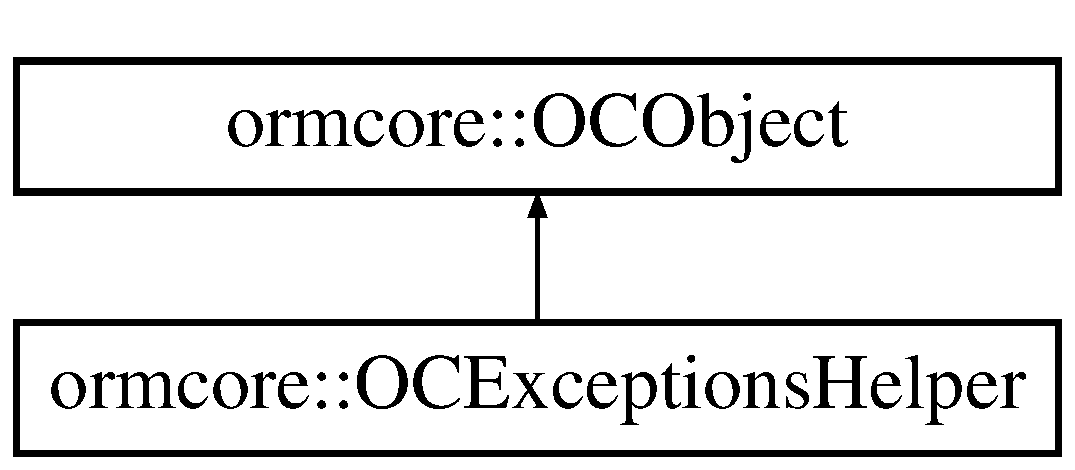
\includegraphics[height=2.000000cm]{classormcore_1_1_o_c_exceptions_helper}
\end{center}
\end{figure}
\subsection*{\-Static \-Public \-Member \-Functions}
\begin{DoxyCompactItemize}
\item 
\hypertarget{classormcore_1_1_o_c_exceptions_helper_ac2c0bc3e1b609386791e0f8a7ce60799}{
static void {\bfseries log\-Exception} (\hyperlink{classormcore_1_1_o_c_s_q_l_exception}{\-O\-C\-S\-Q\-L\-Exception} ex)}
\label{classormcore_1_1_o_c_exceptions_helper_ac2c0bc3e1b609386791e0f8a7ce60799}

\item 
\hypertarget{classormcore_1_1_o_c_exceptions_helper_ad41b6c1cfa856133701562c004a222ff}{
static void {\bfseries log\-Exception} (\hyperlink{classormcore_1_1_o_c_exception}{\-O\-C\-Exception} ex)}
\label{classormcore_1_1_o_c_exceptions_helper_ad41b6c1cfa856133701562c004a222ff}

\end{DoxyCompactItemize}


\-The documentation for this class was generated from the following files\-:\begin{DoxyCompactItemize}
\item 
\-O\-R\-M\-C++/include/ocexceptionshelper.\-h\item 
\-O\-R\-M\-C++/src/ocexceptionshelper.\-cpp\end{DoxyCompactItemize}

\hypertarget{classormcore_1_1_o_c_file_exception}{
\section{ormcore\-:\-:\-O\-C\-File\-Exception \-Class \-Reference}
\label{classormcore_1_1_o_c_file_exception}\index{ormcore\-::\-O\-C\-File\-Exception@{ormcore\-::\-O\-C\-File\-Exception}}
}


{\ttfamily \#include $<$ocfileexception.\-h$>$}

\-Inheritance diagram for ormcore\-:\-:\-O\-C\-File\-Exception\-:\begin{figure}[H]
\begin{center}
\leavevmode
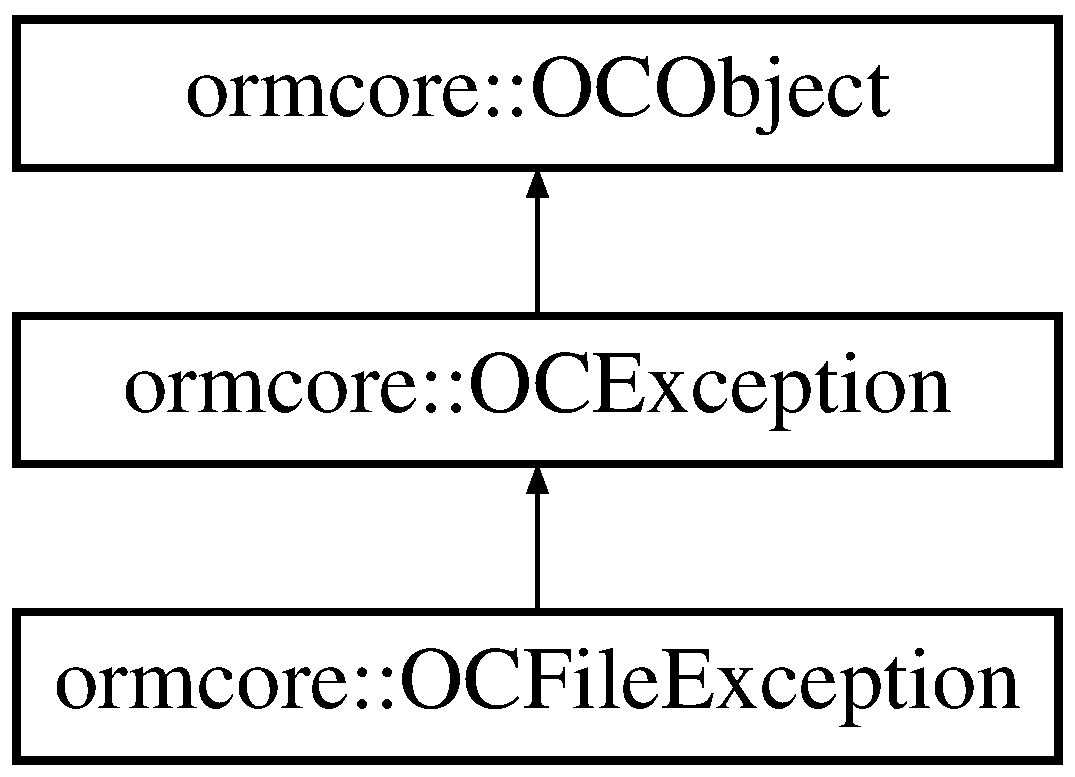
\includegraphics[height=3.000000cm]{classormcore_1_1_o_c_file_exception}
\end{center}
\end{figure}
\subsection*{\-Public \-Member \-Functions}
\begin{DoxyCompactItemize}
\item 
\hyperlink{classormcore_1_1_o_c_file_exception_a834e1e6be5f4c7f3977588c109252e7f}{\-O\-C\-File\-Exception} (\-Q\-String file\-Name, \-Q\-String method\-Name, \-Q\-String message, quint32 line\-No, \-Q\-String file\-Path, \-O\-C\-\_\-\-E\-X\-C\-\_\-\-F\-I\-L\-E operation)
\item 
\-Q\-String \hyperlink{classormcore_1_1_o_c_file_exception_a7ead8200a8458159cba5ffbe8348871c}{file\-Path} ()
\item 
\-Q\-String \hyperlink{classormcore_1_1_o_c_file_exception_a328592db4c7f3ef87ad0332da1e44335}{operation} ()
\end{DoxyCompactItemize}


\subsection{\-Detailed \-Description}
\-Classe para excessões decorrentes da manipulação de arquivos \begin{DoxySeeAlso}{\-See also}
\hyperlink{classormcore_1_1_o_c_exception}{\-O\-C\-Exception} 
\end{DoxySeeAlso}


\subsection{\-Constructor \& \-Destructor \-Documentation}
\hypertarget{classormcore_1_1_o_c_file_exception_a834e1e6be5f4c7f3977588c109252e7f}{
\index{ormcore\-::\-O\-C\-File\-Exception@{ormcore\-::\-O\-C\-File\-Exception}!\-O\-C\-File\-Exception@{\-O\-C\-File\-Exception}}
\index{\-O\-C\-File\-Exception@{\-O\-C\-File\-Exception}!ormcore::OCFileException@{ormcore\-::\-O\-C\-File\-Exception}}
\subsubsection[{\-O\-C\-File\-Exception}]{\setlength{\rightskip}{0pt plus 5cm}ormcore\-::\-O\-C\-File\-Exception\-::\-O\-C\-File\-Exception (
\begin{DoxyParamCaption}
\item[{\-Q\-String}]{file\-Name, }
\item[{\-Q\-String}]{method\-Name, }
\item[{\-Q\-String}]{message, }
\item[{quint32}]{line\-No, }
\item[{\-Q\-String}]{file\-Path, }
\item[{\-O\-C\-\_\-\-E\-X\-C\-\_\-\-F\-I\-L\-E}]{operation}
\end{DoxyParamCaption}
)\hspace{0.3cm}{\ttfamily  \mbox{[}inline\mbox{]}}}}
\label{classormcore_1_1_o_c_file_exception_a834e1e6be5f4c7f3977588c109252e7f}
\-Construtor da classe, com os seguintes parâmetros\-: 
\begin{DoxyParams}{\-Parameters}
{\em file\-Name} & \-Nome do arquivo onde foi gerada a excessão \\
\hline
{\em method\-Name} & \-Nome do método onde foi gerada a excessão \\
\hline
{\em message} & \-Mensagem da excessão gerada \\
\hline
{\em line\-No} & \-Número da linha no arquivo onde foi gerada a excessão \\
\hline
{\em file\-Path} & \-Caminho do arquivo que estava sendo manipulado \\
\hline
{\em operation} & \-Operação que estava sendo executada no arquivo \\
\hline
\end{DoxyParams}


\subsection{\-Member \-Function \-Documentation}
\hypertarget{classormcore_1_1_o_c_file_exception_a7ead8200a8458159cba5ffbe8348871c}{
\index{ormcore\-::\-O\-C\-File\-Exception@{ormcore\-::\-O\-C\-File\-Exception}!file\-Path@{file\-Path}}
\index{file\-Path@{file\-Path}!ormcore::OCFileException@{ormcore\-::\-O\-C\-File\-Exception}}
\subsubsection[{file\-Path}]{\setlength{\rightskip}{0pt plus 5cm}\-Q\-String ormcore\-::\-O\-C\-File\-Exception\-::file\-Path (
\begin{DoxyParamCaption}
{}
\end{DoxyParamCaption}
)\hspace{0.3cm}{\ttfamily  \mbox{[}inline\mbox{]}}}}
\label{classormcore_1_1_o_c_file_exception_a7ead8200a8458159cba5ffbe8348871c}
\begin{DoxyReturn}{\-Returns}
\-O caminho do arquivo que estava sendo manipulado e no qual foi gerada uma excessão 
\end{DoxyReturn}
\hypertarget{classormcore_1_1_o_c_file_exception_a328592db4c7f3ef87ad0332da1e44335}{
\index{ormcore\-::\-O\-C\-File\-Exception@{ormcore\-::\-O\-C\-File\-Exception}!operation@{operation}}
\index{operation@{operation}!ormcore::OCFileException@{ormcore\-::\-O\-C\-File\-Exception}}
\subsubsection[{operation}]{\setlength{\rightskip}{0pt plus 5cm}\-Q\-String ormcore\-::\-O\-C\-File\-Exception\-::operation (
\begin{DoxyParamCaption}
{}
\end{DoxyParamCaption}
)\hspace{0.3cm}{\ttfamily  \mbox{[}inline\mbox{]}}}}
\label{classormcore_1_1_o_c_file_exception_a328592db4c7f3ef87ad0332da1e44335}
\begin{DoxyReturn}{\-Returns}
\-A \-String correnspondente para a operação sendo executada no arquivo no momento da excessão 
\end{DoxyReturn}


\-The documentation for this class was generated from the following file\-:\begin{DoxyCompactItemize}
\item 
\-O\-R\-M\-C++/include/ocfileexception.\-h\end{DoxyCompactItemize}

\hypertarget{classormcore_1_1_o_c_logger}{
\section{ormcore\-:\-:\-O\-C\-Logger \-Class \-Reference}
\label{classormcore_1_1_o_c_logger}\index{ormcore\-::\-O\-C\-Logger@{ormcore\-::\-O\-C\-Logger}}
}


{\ttfamily \#include $<$oclogger.\-h$>$}

\-Inheritance diagram for ormcore\-:\-:\-O\-C\-Logger\-:\begin{figure}[H]
\begin{center}
\leavevmode
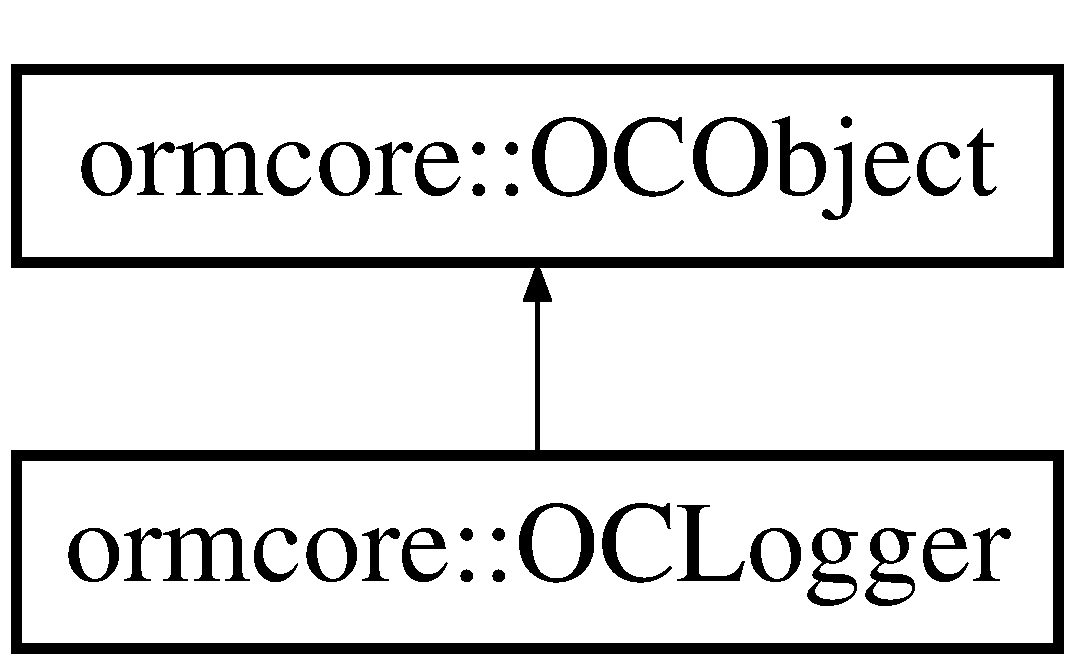
\includegraphics[height=2.000000cm]{classormcore_1_1_o_c_logger}
\end{center}
\end{figure}
\subsection*{\-Static \-Public \-Member \-Functions}
\begin{DoxyCompactItemize}
\item 
static void \hyperlink{classormcore_1_1_o_c_logger_a3459e0daf8528bc1fa6ff2fee8f7ed7b}{init} (const \-Q\-String file\-Name)
\item 
static bool \hyperlink{classormcore_1_1_o_c_logger_a80761cdd34c1c2129781f0e10c49cc13}{is\-Log\-Active} ()
\item 
static void \hyperlink{classormcore_1_1_o_c_logger_a6b4ff14c85dfb0d9a5cfdb5de3e4c810}{set\-Log\-Level} (int log\-Level)
\item 
static void \hyperlink{classormcore_1_1_o_c_logger_a8ad195d1f7324577ab4d0da4c13bb311}{activate\-Debug} (bool activate=true)
\item 
static void \hyperlink{classormcore_1_1_o_c_logger_a0af956315f4126008eb02e38cca14ba7}{end} ()
\item 
static void \hyperlink{classormcore_1_1_o_c_logger_aaa72ada5c6981bc62367d0654f422607}{debug} (\-O\-C\-\_\-\-L\-O\-G\-\_\-\-T\-Y\-P\-E log\-Type, \-Q\-String file, qint32 line, \-Q\-String method, \-Q\-String message)
\end{DoxyCompactItemize}


\subsection{\-Detailed \-Description}
\-Classe que controla o log de mensagens em arquivo ou outros meios 

\subsection{\-Member \-Function \-Documentation}
\hypertarget{classormcore_1_1_o_c_logger_a8ad195d1f7324577ab4d0da4c13bb311}{
\index{ormcore\-::\-O\-C\-Logger@{ormcore\-::\-O\-C\-Logger}!activate\-Debug@{activate\-Debug}}
\index{activate\-Debug@{activate\-Debug}!ormcore::OCLogger@{ormcore\-::\-O\-C\-Logger}}
\subsubsection[{activate\-Debug}]{\setlength{\rightskip}{0pt plus 5cm}static void ormcore\-::\-O\-C\-Logger\-::activate\-Debug (
\begin{DoxyParamCaption}
\item[{bool}]{activate = {\ttfamily true}}
\end{DoxyParamCaption}
)\hspace{0.3cm}{\ttfamily  \mbox{[}inline, static\mbox{]}}}}
\label{classormcore_1_1_o_c_logger_a8ad195d1f7324577ab4d0da4c13bb311}
\-Ativa ou desativa geração de log 
\begin{DoxyParams}{\-Parameters}
{\em is\-Log\-Active} & \-Indica se o log será ativado ou não (true ou false) \\
\hline
\end{DoxyParams}
\hypertarget{classormcore_1_1_o_c_logger_aaa72ada5c6981bc62367d0654f422607}{
\index{ormcore\-::\-O\-C\-Logger@{ormcore\-::\-O\-C\-Logger}!debug@{debug}}
\index{debug@{debug}!ormcore::OCLogger@{ormcore\-::\-O\-C\-Logger}}
\subsubsection[{debug}]{\setlength{\rightskip}{0pt plus 5cm}void \-O\-C\-Logger\-::debug (
\begin{DoxyParamCaption}
\item[{\-O\-C\-\_\-\-L\-O\-G\-\_\-\-T\-Y\-P\-E}]{log\-Type, }
\item[{\-Q\-String}]{file, }
\item[{qint32}]{line, }
\item[{\-Q\-String}]{method, }
\item[{\-Q\-String}]{message}
\end{DoxyParamCaption}
)\hspace{0.3cm}{\ttfamily  \mbox{[}static\mbox{]}}}}
\label{classormcore_1_1_o_c_logger_aaa72ada5c6981bc62367d0654f422607}
\-Registra informações de debug 
\begin{DoxyParams}{\-Parameters}
{\em log\-Type} & \-Tipo da mensagem registrada, podendo ser\-: \-O\-C\-\_\-\-L\-O\-G\-\_\-\-I\-N\-F\-O \-Mensagem apenas informativa. \-O\-C\-\_\-\-L\-O\-G\-\_\-\-W\-A\-R\-N \-Mensagem de alerta, porém não é erro. \-O\-C\-\_\-\-L\-O\-G\-\_\-\-E\-R\-R\-O\-R \-Mensagem de erro, porém não é erro fatal. \-O\-C\-\_\-\-L\-O\-G\-\_\-\-F\-A\-T\-A\-L \-Erro fatal, o programa pode fechar ou apresentar instabilidade. \\
\hline
{\em file} & \-Nome do arquivo fonte que está sendo executado. \\
\hline
{\em line} & \-Linha do arquivo fonte que está sendo executada. \\
\hline
{\em method} & \-Método do programa que está sendo executado. \\
\hline
{\em message} & \-Mensagem a ser registrada no log. \\
\hline
\end{DoxyParams}
\hypertarget{classormcore_1_1_o_c_logger_a0af956315f4126008eb02e38cca14ba7}{
\index{ormcore\-::\-O\-C\-Logger@{ormcore\-::\-O\-C\-Logger}!end@{end}}
\index{end@{end}!ormcore::OCLogger@{ormcore\-::\-O\-C\-Logger}}
\subsubsection[{end}]{\setlength{\rightskip}{0pt plus 5cm}void \-O\-C\-Logger\-::end (
\begin{DoxyParamCaption}
{}
\end{DoxyParamCaption}
)\hspace{0.3cm}{\ttfamily  \mbox{[}static\mbox{]}}}}
\label{classormcore_1_1_o_c_logger_a0af956315f4126008eb02e38cca14ba7}
\-Encerra gravação do log \hypertarget{classormcore_1_1_o_c_logger_a3459e0daf8528bc1fa6ff2fee8f7ed7b}{
\index{ormcore\-::\-O\-C\-Logger@{ormcore\-::\-O\-C\-Logger}!init@{init}}
\index{init@{init}!ormcore::OCLogger@{ormcore\-::\-O\-C\-Logger}}
\subsubsection[{init}]{\setlength{\rightskip}{0pt plus 5cm}void \-O\-C\-Logger\-::init (
\begin{DoxyParamCaption}
\item[{const \-Q\-String}]{file\-Name}
\end{DoxyParamCaption}
)\hspace{0.3cm}{\ttfamily  \mbox{[}static\mbox{]}}}}
\label{classormcore_1_1_o_c_logger_a3459e0daf8528bc1fa6ff2fee8f7ed7b}
\-Inicializa registro do log 
\begin{DoxyParams}{\-Parameters}
{\em file\-Name} & \-Nome do arquivo para onde serão registradas as mensagens \\
\hline
\end{DoxyParams}
\hypertarget{classormcore_1_1_o_c_logger_a80761cdd34c1c2129781f0e10c49cc13}{
\index{ormcore\-::\-O\-C\-Logger@{ormcore\-::\-O\-C\-Logger}!is\-Log\-Active@{is\-Log\-Active}}
\index{is\-Log\-Active@{is\-Log\-Active}!ormcore::OCLogger@{ormcore\-::\-O\-C\-Logger}}
\subsubsection[{is\-Log\-Active}]{\setlength{\rightskip}{0pt plus 5cm}static bool ormcore\-::\-O\-C\-Logger\-::is\-Log\-Active (
\begin{DoxyParamCaption}
{}
\end{DoxyParamCaption}
)\hspace{0.3cm}{\ttfamily  \mbox{[}inline, static\mbox{]}}}}
\label{classormcore_1_1_o_c_logger_a80761cdd34c1c2129781f0e10c49cc13}
\begin{DoxyReturn}{\-Returns}
\-Se debug está ativo ou não 
\end{DoxyReturn}
\hypertarget{classormcore_1_1_o_c_logger_a6b4ff14c85dfb0d9a5cfdb5de3e4c810}{
\index{ormcore\-::\-O\-C\-Logger@{ormcore\-::\-O\-C\-Logger}!set\-Log\-Level@{set\-Log\-Level}}
\index{set\-Log\-Level@{set\-Log\-Level}!ormcore::OCLogger@{ormcore\-::\-O\-C\-Logger}}
\subsubsection[{set\-Log\-Level}]{\setlength{\rightskip}{0pt plus 5cm}static void ormcore\-::\-O\-C\-Logger\-::set\-Log\-Level (
\begin{DoxyParamCaption}
\item[{int}]{log\-Level}
\end{DoxyParamCaption}
)\hspace{0.3cm}{\ttfamily  \mbox{[}inline, static\mbox{]}}}}
\label{classormcore_1_1_o_c_logger_a6b4ff14c85dfb0d9a5cfdb5de3e4c810}
\-Atribui o nível mínimo de log (-\/1 para todos os níveis) 
\begin{DoxyParams}{\-Parameters}
{\em log\-Level} & \-O nível de log a ser mostrado \\
\hline
\end{DoxyParams}


\-The documentation for this class was generated from the following files\-:\begin{DoxyCompactItemize}
\item 
\-O\-R\-M\-C++/include/oclogger.\-h\item 
\-O\-R\-M\-C++/src/oclogger.\-cpp\end{DoxyCompactItemize}

\hypertarget{classormcore_1_1_o_c_model}{
\section{ormcore\-:\-:\-O\-C\-Model \-Class \-Reference}
\label{classormcore_1_1_o_c_model}\index{ormcore\-::\-O\-C\-Model@{ormcore\-::\-O\-C\-Model}}
}


{\ttfamily \#include $<$ocmodel.\-h$>$}

\-Inheritance diagram for ormcore\-:\-:\-O\-C\-Model\-:\begin{figure}[H]
\begin{center}
\leavevmode
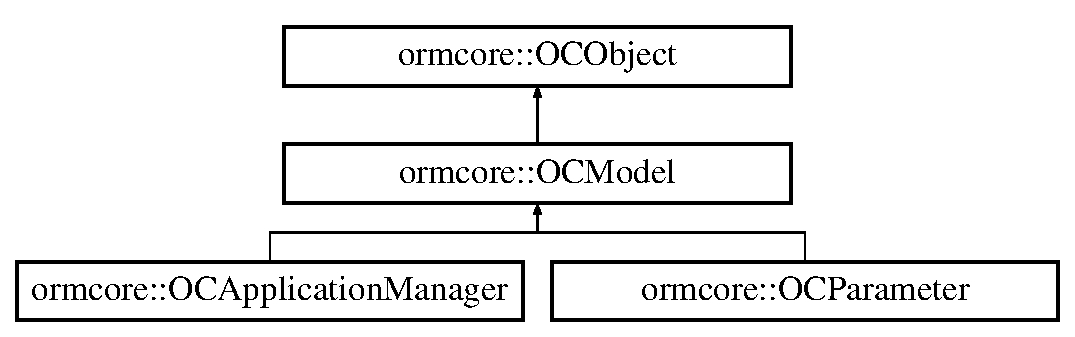
\includegraphics[height=3.000000cm]{classormcore_1_1_o_c_model}
\end{center}
\end{figure}
\subsection*{\-Public \-Member \-Functions}
\begin{DoxyCompactItemize}
\item 
\hyperlink{classormcore_1_1_o_c_model_af71a4d619bede3a8701c273ca0558c29}{\-O\-C\-Model} ()
\item 
quint64 \hyperlink{classormcore_1_1_o_c_model_a5ea297130eecaa9bc7eab2e0c4a743a1}{id} ()
\item 
void \hyperlink{classormcore_1_1_o_c_model_ac8287eb78aa18392a0231b71fa66b450}{set\-Id} (quint64 id)
\item 
\-Q\-Hash$<$ \-Q\-String, \-Q\-Variant $>$ \& \hyperlink{classormcore_1_1_o_c_model_aa58346d1a59a995e598389d8b8ea2b5b}{table\-Fields} ()
\end{DoxyCompactItemize}
\subsection*{\-Static \-Public \-Attributes}
\begin{DoxyCompactItemize}
\item 
\hypertarget{classormcore_1_1_o_c_model_adbcc25b105925536f1eb1c1b6d96d4db}{
static \-Q\-String {\bfseries \-\_\-table\-Name} = \char`\"{}\char`\"{}}
\label{classormcore_1_1_o_c_model_adbcc25b105925536f1eb1c1b6d96d4db}

\item 
\hypertarget{classormcore_1_1_o_c_model_adc7c45bf12c6ab0b5b025038d9b3817d}{
static \-Q\-String {\bfseries \-\_\-full\-Schema} = \char`\"{}\char`\"{}}
\label{classormcore_1_1_o_c_model_adc7c45bf12c6ab0b5b025038d9b3817d}

\end{DoxyCompactItemize}


\subsection{\-Detailed \-Description}
\-Classe manipulação de objetos do banco de dados 

\subsection{\-Constructor \& \-Destructor \-Documentation}
\hypertarget{classormcore_1_1_o_c_model_af71a4d619bede3a8701c273ca0558c29}{
\index{ormcore\-::\-O\-C\-Model@{ormcore\-::\-O\-C\-Model}!\-O\-C\-Model@{\-O\-C\-Model}}
\index{\-O\-C\-Model@{\-O\-C\-Model}!ormcore::OCModel@{ormcore\-::\-O\-C\-Model}}
\subsubsection[{\-O\-C\-Model}]{\setlength{\rightskip}{0pt plus 5cm}\-O\-C\-Model\-::\-O\-C\-Model (
\begin{DoxyParamCaption}
{}
\end{DoxyParamCaption}
)}}
\label{classormcore_1_1_o_c_model_af71a4d619bede3a8701c273ca0558c29}
\-Construtor da classe 

\subsection{\-Member \-Function \-Documentation}
\hypertarget{classormcore_1_1_o_c_model_a5ea297130eecaa9bc7eab2e0c4a743a1}{
\index{ormcore\-::\-O\-C\-Model@{ormcore\-::\-O\-C\-Model}!id@{id}}
\index{id@{id}!ormcore::OCModel@{ormcore\-::\-O\-C\-Model}}
\subsubsection[{id}]{\setlength{\rightskip}{0pt plus 5cm}quint64 ormcore\-::\-O\-C\-Model\-::id (
\begin{DoxyParamCaption}
{}
\end{DoxyParamCaption}
)\hspace{0.3cm}{\ttfamily  \mbox{[}inline\mbox{]}}}}
\label{classormcore_1_1_o_c_model_a5ea297130eecaa9bc7eab2e0c4a743a1}
\begin{DoxyReturn}{\-Returns}
id do objeto 
\end{DoxyReturn}
\hypertarget{classormcore_1_1_o_c_model_ac8287eb78aa18392a0231b71fa66b450}{
\index{ormcore\-::\-O\-C\-Model@{ormcore\-::\-O\-C\-Model}!set\-Id@{set\-Id}}
\index{set\-Id@{set\-Id}!ormcore::OCModel@{ormcore\-::\-O\-C\-Model}}
\subsubsection[{set\-Id}]{\setlength{\rightskip}{0pt plus 5cm}void ormcore\-::\-O\-C\-Model\-::set\-Id (
\begin{DoxyParamCaption}
\item[{quint64}]{id}
\end{DoxyParamCaption}
)\hspace{0.3cm}{\ttfamily  \mbox{[}inline\mbox{]}}}}
\label{classormcore_1_1_o_c_model_ac8287eb78aa18392a0231b71fa66b450}
\-Atribui o id do objeto 
\begin{DoxyParams}{\-Parameters}
{\em id} & \-Id do objeto \\
\hline
\end{DoxyParams}
\hypertarget{classormcore_1_1_o_c_model_aa58346d1a59a995e598389d8b8ea2b5b}{
\index{ormcore\-::\-O\-C\-Model@{ormcore\-::\-O\-C\-Model}!table\-Fields@{table\-Fields}}
\index{table\-Fields@{table\-Fields}!ormcore::OCModel@{ormcore\-::\-O\-C\-Model}}
\subsubsection[{table\-Fields}]{\setlength{\rightskip}{0pt plus 5cm}\-Q\-Hash$<$\-Q\-String, \-Q\-Variant$>$\& ormcore\-::\-O\-C\-Model\-::table\-Fields (
\begin{DoxyParamCaption}
{}
\end{DoxyParamCaption}
)\hspace{0.3cm}{\ttfamily  \mbox{[}inline\mbox{]}}}}
\label{classormcore_1_1_o_c_model_aa58346d1a59a995e598389d8b8ea2b5b}
\begin{DoxyReturn}{\-Returns}
\-Campos da tabela na forma de hash table 
\end{DoxyReturn}


\-The documentation for this class was generated from the following files\-:\begin{DoxyCompactItemize}
\item 
\-O\-R\-M\-C++/include/ocmodel.\-h\item 
\-O\-R\-M\-C++/src/ocmodel.\-cpp\end{DoxyCompactItemize}

\hypertarget{classormcore_1_1_o_c_object}{
\section{ormcore\-:\-:\-O\-C\-Object \-Class \-Reference}
\label{classormcore_1_1_o_c_object}\index{ormcore\-::\-O\-C\-Object@{ormcore\-::\-O\-C\-Object}}
}


{\ttfamily \#include $<$ocobject.\-h$>$}

\-Inheritance diagram for ormcore\-:\-:\-O\-C\-Object\-:\begin{figure}[H]
\begin{center}
\leavevmode
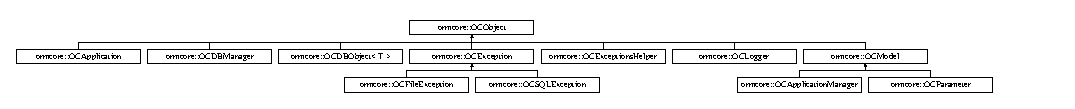
\includegraphics[height=1.019417cm]{classormcore_1_1_o_c_object}
\end{center}
\end{figure}
\subsection*{\-Public \-Member \-Functions}
\begin{DoxyCompactItemize}
\item 
\hyperlink{classormcore_1_1_o_c_object_ac0632af27fd5eba7dc3d51374ce69786}{\-O\-C\-Object} (\-Q\-String name=\char`\"{}\-O\-C\-Object\char`\"{})
\end{DoxyCompactItemize}


\subsection{\-Detailed \-Description}
\-Classe abstrata da qual todos as classes do projeto devem herdar 

\subsection{\-Constructor \& \-Destructor \-Documentation}
\hypertarget{classormcore_1_1_o_c_object_ac0632af27fd5eba7dc3d51374ce69786}{
\index{ormcore\-::\-O\-C\-Object@{ormcore\-::\-O\-C\-Object}!\-O\-C\-Object@{\-O\-C\-Object}}
\index{\-O\-C\-Object@{\-O\-C\-Object}!ormcore::OCObject@{ormcore\-::\-O\-C\-Object}}
\subsubsection[{\-O\-C\-Object}]{\setlength{\rightskip}{0pt plus 5cm}\-O\-C\-Object\-::\-O\-C\-Object (
\begin{DoxyParamCaption}
\item[{\-Q\-String}]{name = {\ttfamily \char`\"{}\-O\-C\-Object\char`\"{}}}
\end{DoxyParamCaption}
)}}
\label{classormcore_1_1_o_c_object_ac0632af27fd5eba7dc3d51374ce69786}
\-Construtor da classe 
\begin{DoxyParams}{\-Parameters}
{\em name} & \-Nome da classe como metainformação \\
\hline
\end{DoxyParams}


\-The documentation for this class was generated from the following files\-:\begin{DoxyCompactItemize}
\item 
\-O\-R\-M\-C++/include/ocobject.\-h\item 
\-O\-R\-M\-C++/src/ocobject.\-cpp\end{DoxyCompactItemize}

\hypertarget{classormcore_1_1_o_c_parameter}{
\section{ormcore\-:\-:\-O\-C\-Parameter \-Class \-Reference}
\label{classormcore_1_1_o_c_parameter}\index{ormcore\-::\-O\-C\-Parameter@{ormcore\-::\-O\-C\-Parameter}}
}
\-Inheritance diagram for ormcore\-:\-:\-O\-C\-Parameter\-:\begin{figure}[H]
\begin{center}
\leavevmode
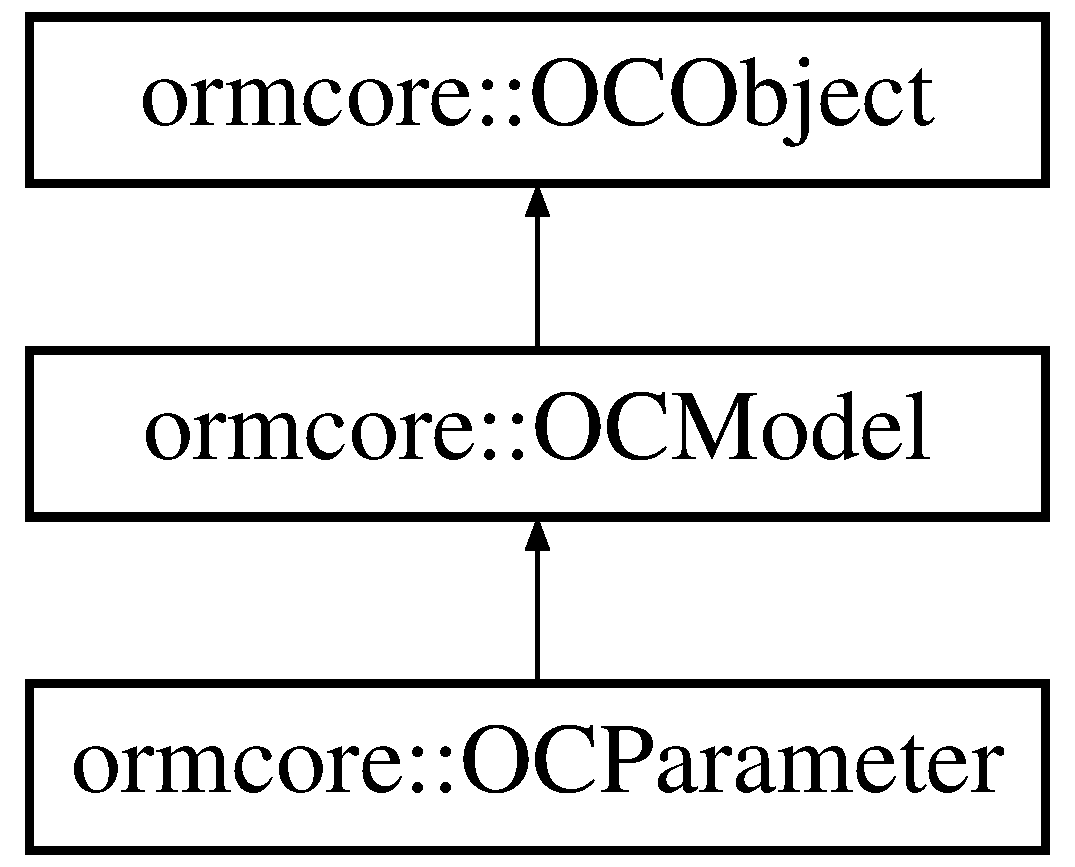
\includegraphics[height=3.000000cm]{classormcore_1_1_o_c_parameter}
\end{center}
\end{figure}
\subsection*{\-Public \-Member \-Functions}
\begin{DoxyCompactItemize}
\item 
\hyperlink{classormcore_1_1_o_c_parameter_a4c009b883c11052314c288620615da43}{\-O\-C\-Parameter} ()
\end{DoxyCompactItemize}
\subsection*{\-Static \-Public \-Attributes}
\begin{DoxyCompactItemize}
\item 
\hypertarget{classormcore_1_1_o_c_parameter_a4328bfaee523058a71bbb44f0f134093}{
static \-Q\-String {\bfseries \-\_\-full\-Schema} = \char`\"{}item\-Order \-I\-N\-T\-E\-G\-E\-R\char`\"{}}
\label{classormcore_1_1_o_c_parameter_a4328bfaee523058a71bbb44f0f134093}

\item 
\hypertarget{classormcore_1_1_o_c_parameter_ac782f4af1a6ed5345a9f9fd30f5e0efb}{
static \-Q\-String {\bfseries \-\_\-table\-Name} = \char`\"{}parameter\char`\"{}}
\label{classormcore_1_1_o_c_parameter_ac782f4af1a6ed5345a9f9fd30f5e0efb}

\end{DoxyCompactItemize}


\subsection{\-Constructor \& \-Destructor \-Documentation}
\hypertarget{classormcore_1_1_o_c_parameter_a4c009b883c11052314c288620615da43}{
\index{ormcore\-::\-O\-C\-Parameter@{ormcore\-::\-O\-C\-Parameter}!\-O\-C\-Parameter@{\-O\-C\-Parameter}}
\index{\-O\-C\-Parameter@{\-O\-C\-Parameter}!ormcore::OCParameter@{ormcore\-::\-O\-C\-Parameter}}
\subsubsection[{\-O\-C\-Parameter}]{\setlength{\rightskip}{0pt plus 5cm}\-O\-C\-Parameter\-::\-O\-C\-Parameter (
\begin{DoxyParamCaption}
{}
\end{DoxyParamCaption}
)}}
\label{classormcore_1_1_o_c_parameter_a4c009b883c11052314c288620615da43}
\-Construtor de \hyperlink{classormcore_1_1_o_c_parameter}{\-O\-C\-Parameter} 

\-The documentation for this class was generated from the following files\-:\begin{DoxyCompactItemize}
\item 
\-O\-R\-M\-C++/include/ocparameter.\-h\item 
\-O\-R\-M\-C++/src/ocparameter.\-cpp\end{DoxyCompactItemize}

\hypertarget{classormcore_1_1_o_c_s_q_l_exception}{
\section{ormcore\-:\-:\-O\-C\-S\-Q\-L\-Exception \-Class \-Reference}
\label{classormcore_1_1_o_c_s_q_l_exception}\index{ormcore\-::\-O\-C\-S\-Q\-L\-Exception@{ormcore\-::\-O\-C\-S\-Q\-L\-Exception}}
}


{\ttfamily \#include $<$ocsqlexception.\-h$>$}

\-Inheritance diagram for ormcore\-:\-:\-O\-C\-S\-Q\-L\-Exception\-:\begin{figure}[H]
\begin{center}
\leavevmode
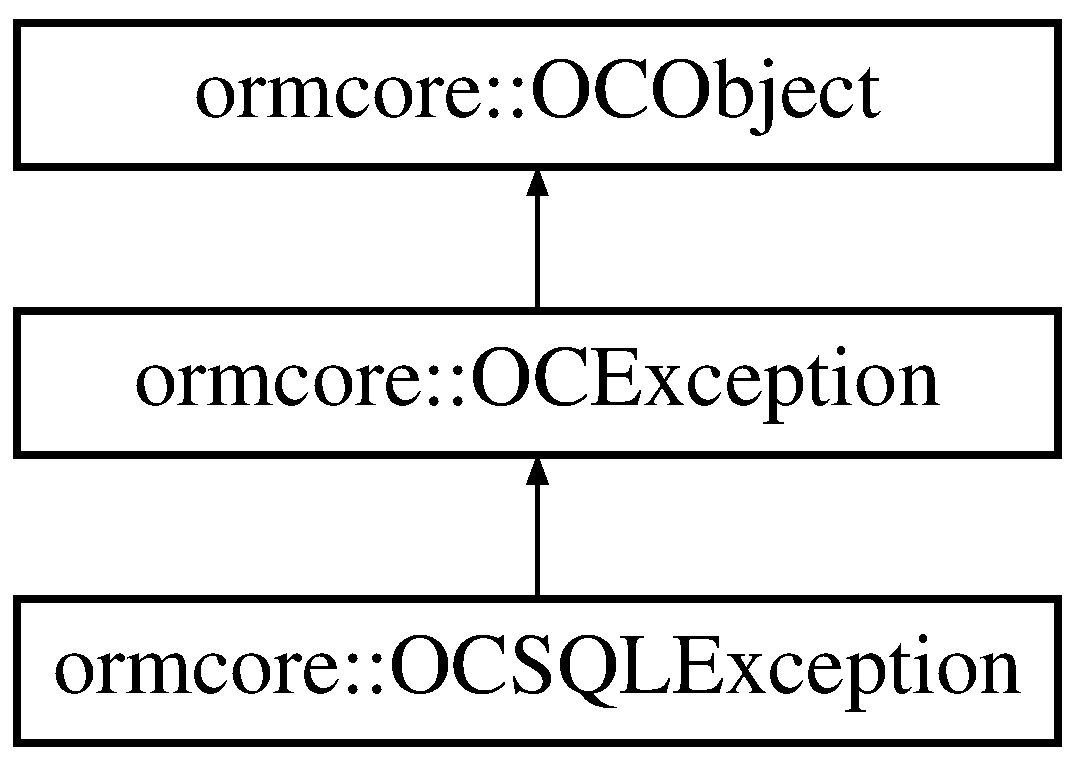
\includegraphics[height=3.000000cm]{classormcore_1_1_o_c_s_q_l_exception}
\end{center}
\end{figure}
\subsection*{\-Public \-Member \-Functions}
\begin{DoxyCompactItemize}
\item 
\hypertarget{classormcore_1_1_o_c_s_q_l_exception_abf284ac4fb4dcba3150f4c6e1b0d7f5f}{
{\bfseries \-O\-C\-S\-Q\-L\-Exception} (\-Q\-String file\-Name, \-Q\-String method\-Name, \-Q\-String message, quint32 line\-No, \-Q\-String db\-Name, \-Q\-String sql\-Query, \-Q\-Sql\-Error sql\-Error)}
\label{classormcore_1_1_o_c_s_q_l_exception_abf284ac4fb4dcba3150f4c6e1b0d7f5f}

\item 
\-Q\-String \hyperlink{classormcore_1_1_o_c_s_q_l_exception_af33c17bf8f9000c94d95c575c63cf936}{db\-Name} ()
\item 
\hypertarget{classormcore_1_1_o_c_s_q_l_exception_a14dc3b97c291099365e39ef4d728dcdb}{
\-Q\-String {\bfseries sql\-Query} ()}
\label{classormcore_1_1_o_c_s_q_l_exception_a14dc3b97c291099365e39ef4d728dcdb}

\item 
\hypertarget{classormcore_1_1_o_c_s_q_l_exception_a880f542cc6f79f49115b429228cc7a82}{
\-Q\-Sql\-Error {\bfseries sql\-Error} ()}
\label{classormcore_1_1_o_c_s_q_l_exception_a880f542cc6f79f49115b429228cc7a82}

\end{DoxyCompactItemize}


\subsection{\-Detailed \-Description}
\-Classe de exceções relacionadas a comandos \-S\-Q\-L e acesso ao banco de dados. 

\subsection{\-Member \-Function \-Documentation}
\hypertarget{classormcore_1_1_o_c_s_q_l_exception_af33c17bf8f9000c94d95c575c63cf936}{
\index{ormcore\-::\-O\-C\-S\-Q\-L\-Exception@{ormcore\-::\-O\-C\-S\-Q\-L\-Exception}!db\-Name@{db\-Name}}
\index{db\-Name@{db\-Name}!ormcore::OCSQLException@{ormcore\-::\-O\-C\-S\-Q\-L\-Exception}}
\subsubsection[{db\-Name}]{\setlength{\rightskip}{0pt plus 5cm}\-Q\-String ormcore\-::\-O\-C\-S\-Q\-L\-Exception\-::db\-Name (
\begin{DoxyParamCaption}
{}
\end{DoxyParamCaption}
)\hspace{0.3cm}{\ttfamily  \mbox{[}inline\mbox{]}}}}
\label{classormcore_1_1_o_c_s_q_l_exception_af33c17bf8f9000c94d95c575c63cf936}
\begin{DoxyReturn}{\-Returns}
\-Nome do banco de dados que está conectado. 

\-Query \-S\-Q\-L que estava sendo executada. 

\-Ultimo erro de \-S\-Q\-L ocorrido. 
\end{DoxyReturn}


\-The documentation for this class was generated from the following file\-:\begin{DoxyCompactItemize}
\item 
\-O\-R\-M\-C++/include/ocsqlexception.\-h\end{DoxyCompactItemize}

\hypertarget{class_o_r_m_c_u_t_test}{
\section{\-O\-R\-M\-C\-U\-T\-Test \-Class \-Reference}
\label{class_o_r_m_c_u_t_test}\index{\-O\-R\-M\-C\-U\-T\-Test@{\-O\-R\-M\-C\-U\-T\-Test}}
}


\-The documentation for this class was generated from the following file\-:\begin{DoxyCompactItemize}
\item 
\-O\-R\-M\-C++\-U\-T/tst\-\_\-ormctest.\-cpp\end{DoxyCompactItemize}

\printindex
\end{document}
